
%%%%%%%%%%%%%%%%%%%%%%%%%%%%%%%%%%%%%%%%%
%\section{Validation of Fit Model} 

%\subsection{Validation of the Fit Model Using Pseudo Data}
%\begin{itemize} 
%\item Any intrinsic bias(sanity check) : Is there any background 
%      whose normalization is biased or constrained too much by fit?
%\item If one bkgd is biased, is it covered by fit? 
%\item What are the most constrained nuisances?  There are some WW-related nuisances   
%that are constrained by a lot, so need to make sure that our fit model fits data correctly 
%(this is a summary of this subsection, and at the same time an introduction to the next section)
%\end{itemize} 

\section{Validation of the Fit Model Using Real Data}

In the shape-based method, we rely on simulation for the background shapes 
except \Wjets. Therefore, it is important to confirm that our fit model,
both shape and normalization, correctly describes what is observed in data. 

The idea is to choose a control region which is dominated by (a) process(es) 
under study, and to fit the region using our fit model.  
If the fit model is not correct then the post-fit shape 
and normalization would not describe the data correctly, 
\textit{i.e.} difference between data and the post-fit shape and normalization
would be large. 

This section describes the validation of fit model of dominant backgrounds, 
\qqww, \topbkg, \Wjets\ and \wgamma/\wgammastar, using dedicated control regions. 

%%%%%%%%%%%%%%%%%%%%%%%%%%%%%%%%%%%%%%%%%%%
\subsection{Validation of \qqww\ fit model}  

The most sensitive channel, 0-jet \DF, is dominated by the $qq\rightarrow\WW$ background. 
Therefore validating the $qq\rightarrow\WW$ fit model is crucial. 
This section describes a validation study using two 
control regions dominated by $qq\rightarrow\WW$ events.
The basic idea is that if the fit model is not correct then the prediction using 
one region may not be compatible with that using another region. To test this, 
we use the post-fit result in one control region, and predict the shape 
and the normalization in another region. 
Following is the procedure and the result of this test. 

We first select two control regions with similar statistics. It is important that 
both regions have a similar number of events so that they have a similar statistical 
power to constrain backgrounds. 
%
\begin{figure}[!hbtp]
\centering
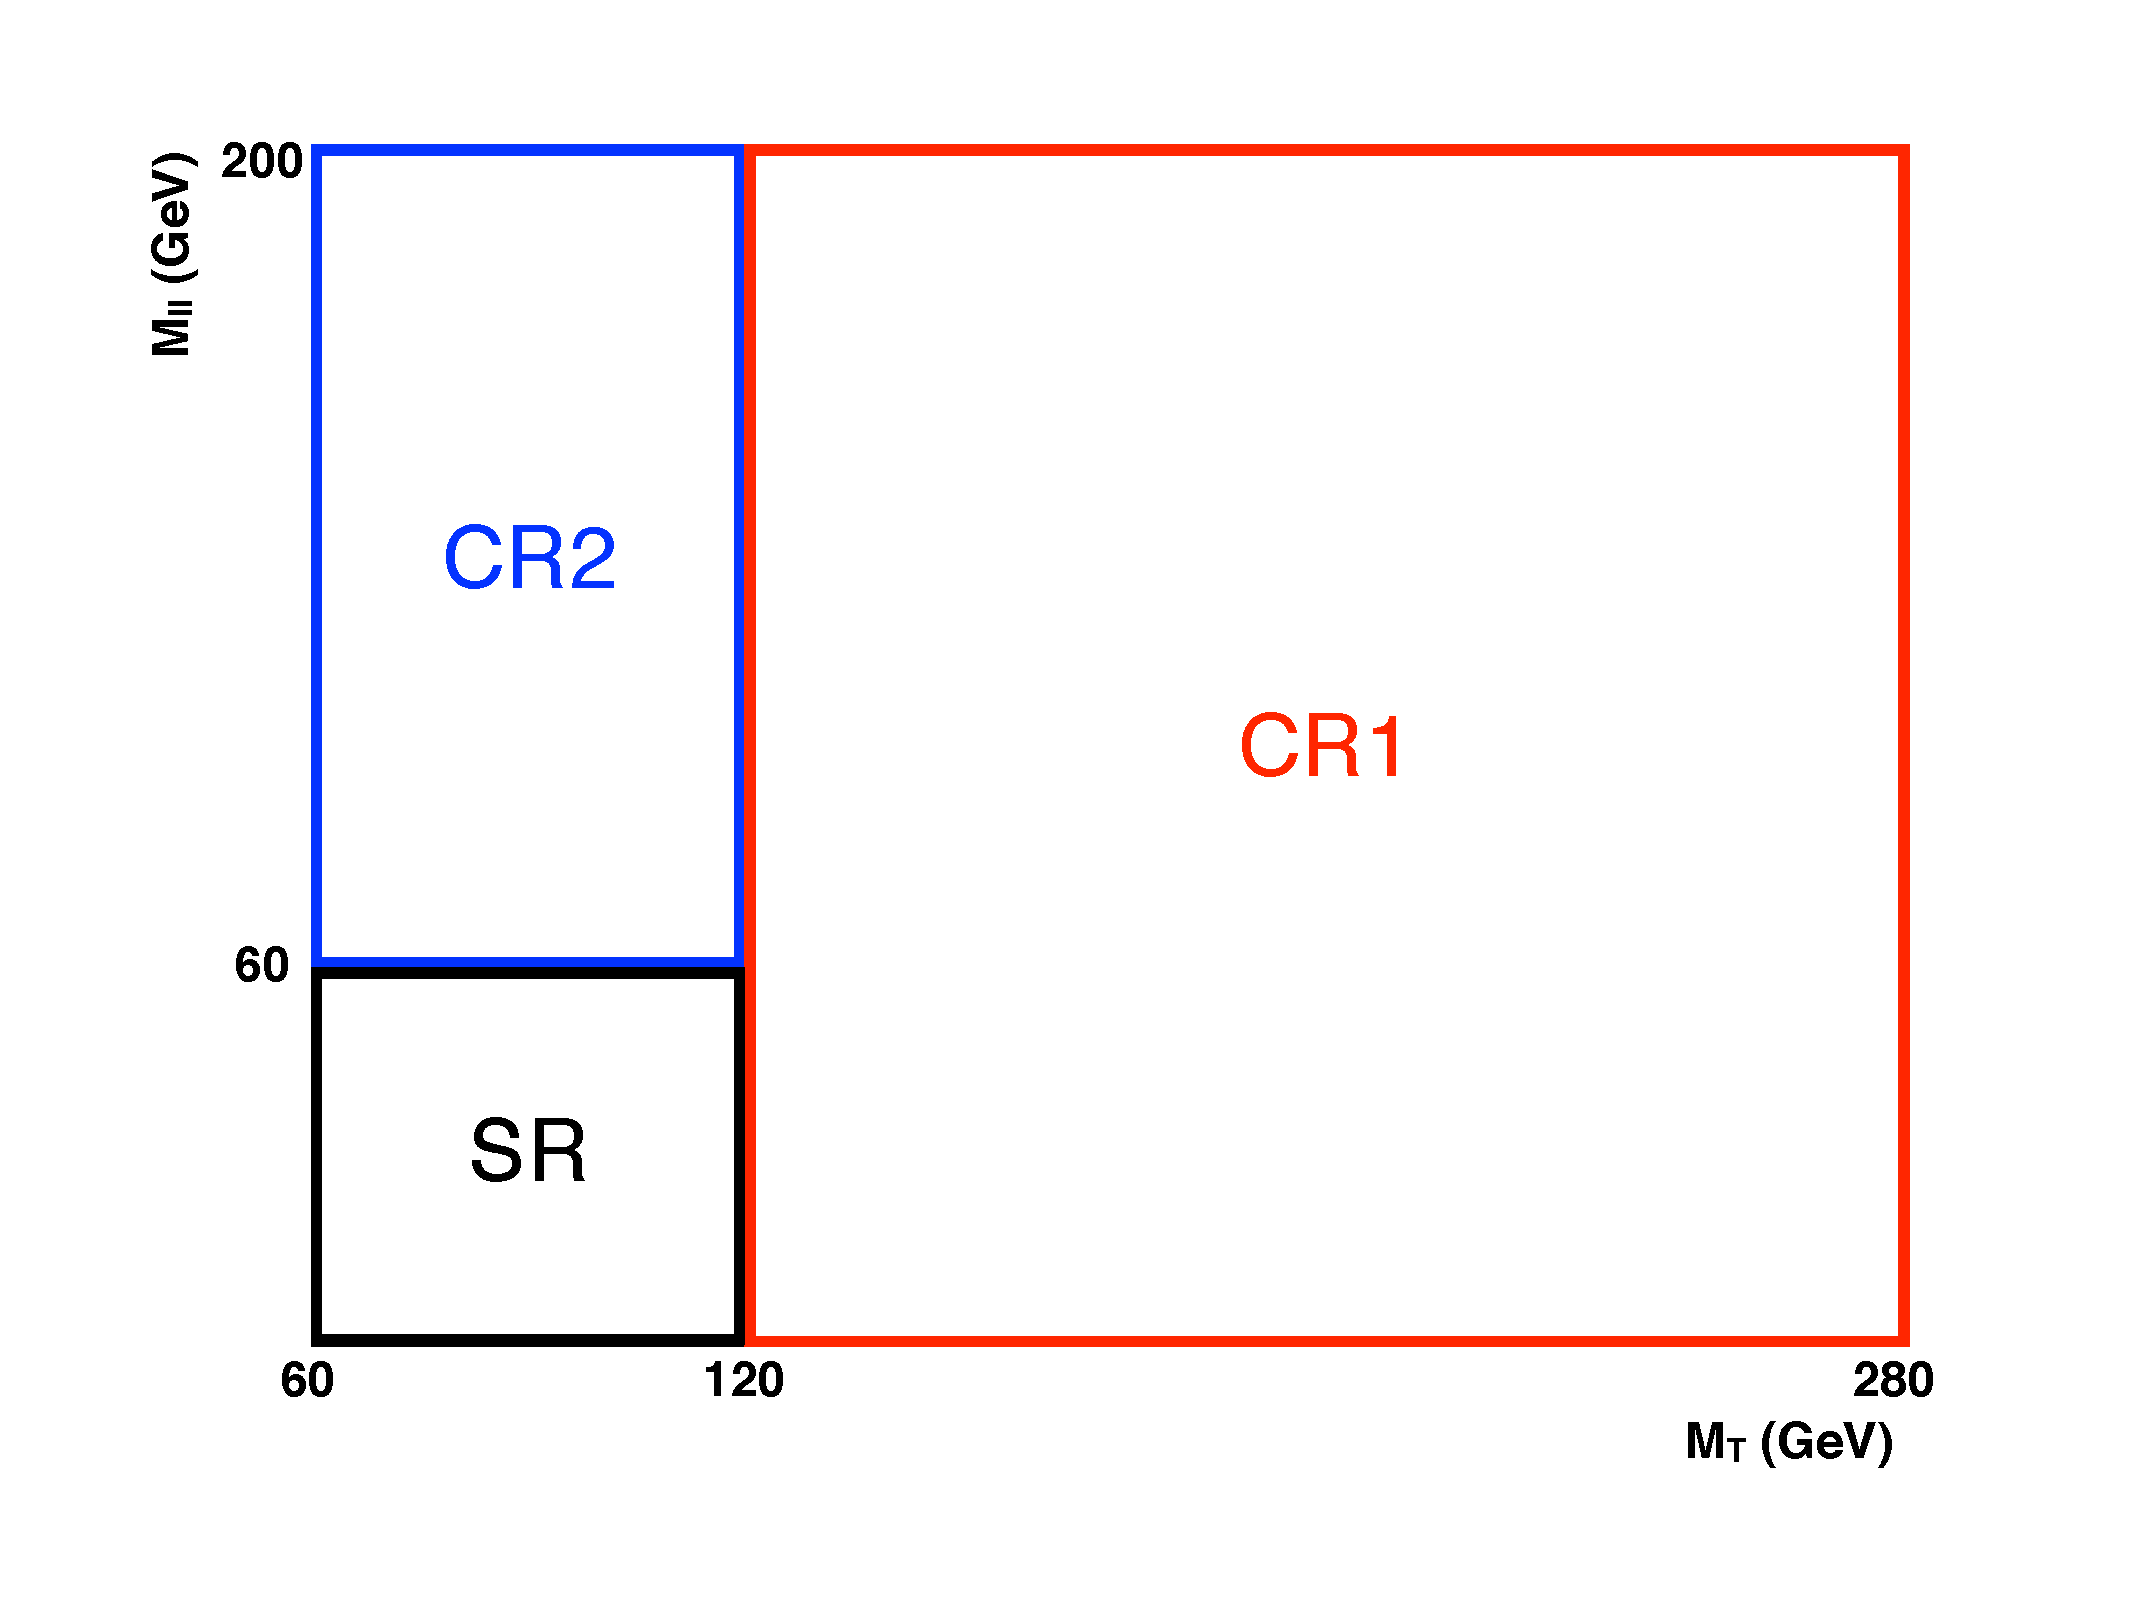
\includegraphics[width=.6\textwidth]{figures/WWctl_scheme.pdf}
\caption{Definition of signal region(SR), and two control regions(CR1 and CR2). 
SR is defined by $60<\mT<120~\GeV$ and $12<\mll<60~\GeV$. 
CR1 is defined by $120<\mT<280~\GeV$ and $12<\mll<200~\GeV$ and 
CR2 is defined by $60<\mT<120~\GeV$ and $60<\mll<200~\GeV$. }
\label{fig:WWctlregions}
\end{figure}
Figure \ref{fig:WWctlregions} shows signal region(SR) which is drawn in black 
and two control regions, CR1 and CR2, which are drawn in red and in blue, respectively. 
The SR is defined as $60<\mT<120~\GeV$ and $12<\mll<60~\GeV$. 
The CR1 is defined as $120<\mT<280~\GeV$ and $12<\mll<200~\GeV$, 
and the CR2 is defined as $60<\mT<120~\GeV$ and $60<\mll<200~\GeV$. 
%
\begin{table}
\footnotesize
\begin{center}
\begin{tabular}{c|ccccc|c}
\hline
Region      & Signal & \qqww & \ggww & \vv & \topbkg &  \\
\hline
CR1         & 27.0  &  1321.0 & 113.2 &  46.2  &  289.6 & \\ 
CR2         & 13.5  &  1672.7 & 54.5  &  51.5  &  146.1 & \\ 
Full range  & 238.4 &  3969.6 & 210.6 &  132.6 &  498.7 & \\ 
\hline
Region      & \WjetsE & \WjetsM & \wgamma & \wgammastar & \ztt & Data \\
\hline
CR1         &  54.9  &  22.4  &   6.0   & 19.3  &   2.8 &   1892\\
CR2         &  108.1 &  128.2 &  19.3   & 21.4  &  19.9 &   2155 \\
Full range  &  282.8 &  331.8 &  115.6  & 167.8 &  46.0 &   5729 \\
\hline
\end{tabular}
\end{center}
\caption{Definition of signal region(SR), and two control regions(CR1 and CR2).} 
\label{tab:WWctlregions_composition}
\end{table}
The composition of signal and backgrounds in the two control regions is summarized 
in Table \ref{tab:WWctlregions_composition}. Both regions are dominated by \qqww  
with purity of around 70(75)\% in CR1(2). 
The signal contamination is negligible(less than 1.5\%) in both regions. 

Because this test is only for \qqww, other processes have to be fixed in the fit.
Therefore, all other processes are fixed to the post-fit normalization and shape 
of the nominal fit except $qq\rightarrow\WW$ process. 
Hereafter, this configuration will be called ``full range" fit. 
In the full range fit, all nuisances for $qq\rightarrow\WW$ are included, 
but all nuisances for other processes are dropped because 
shape and normalization for those processes are already post-fit results. 
%
\begin{figure}[!hbtp]
\centering
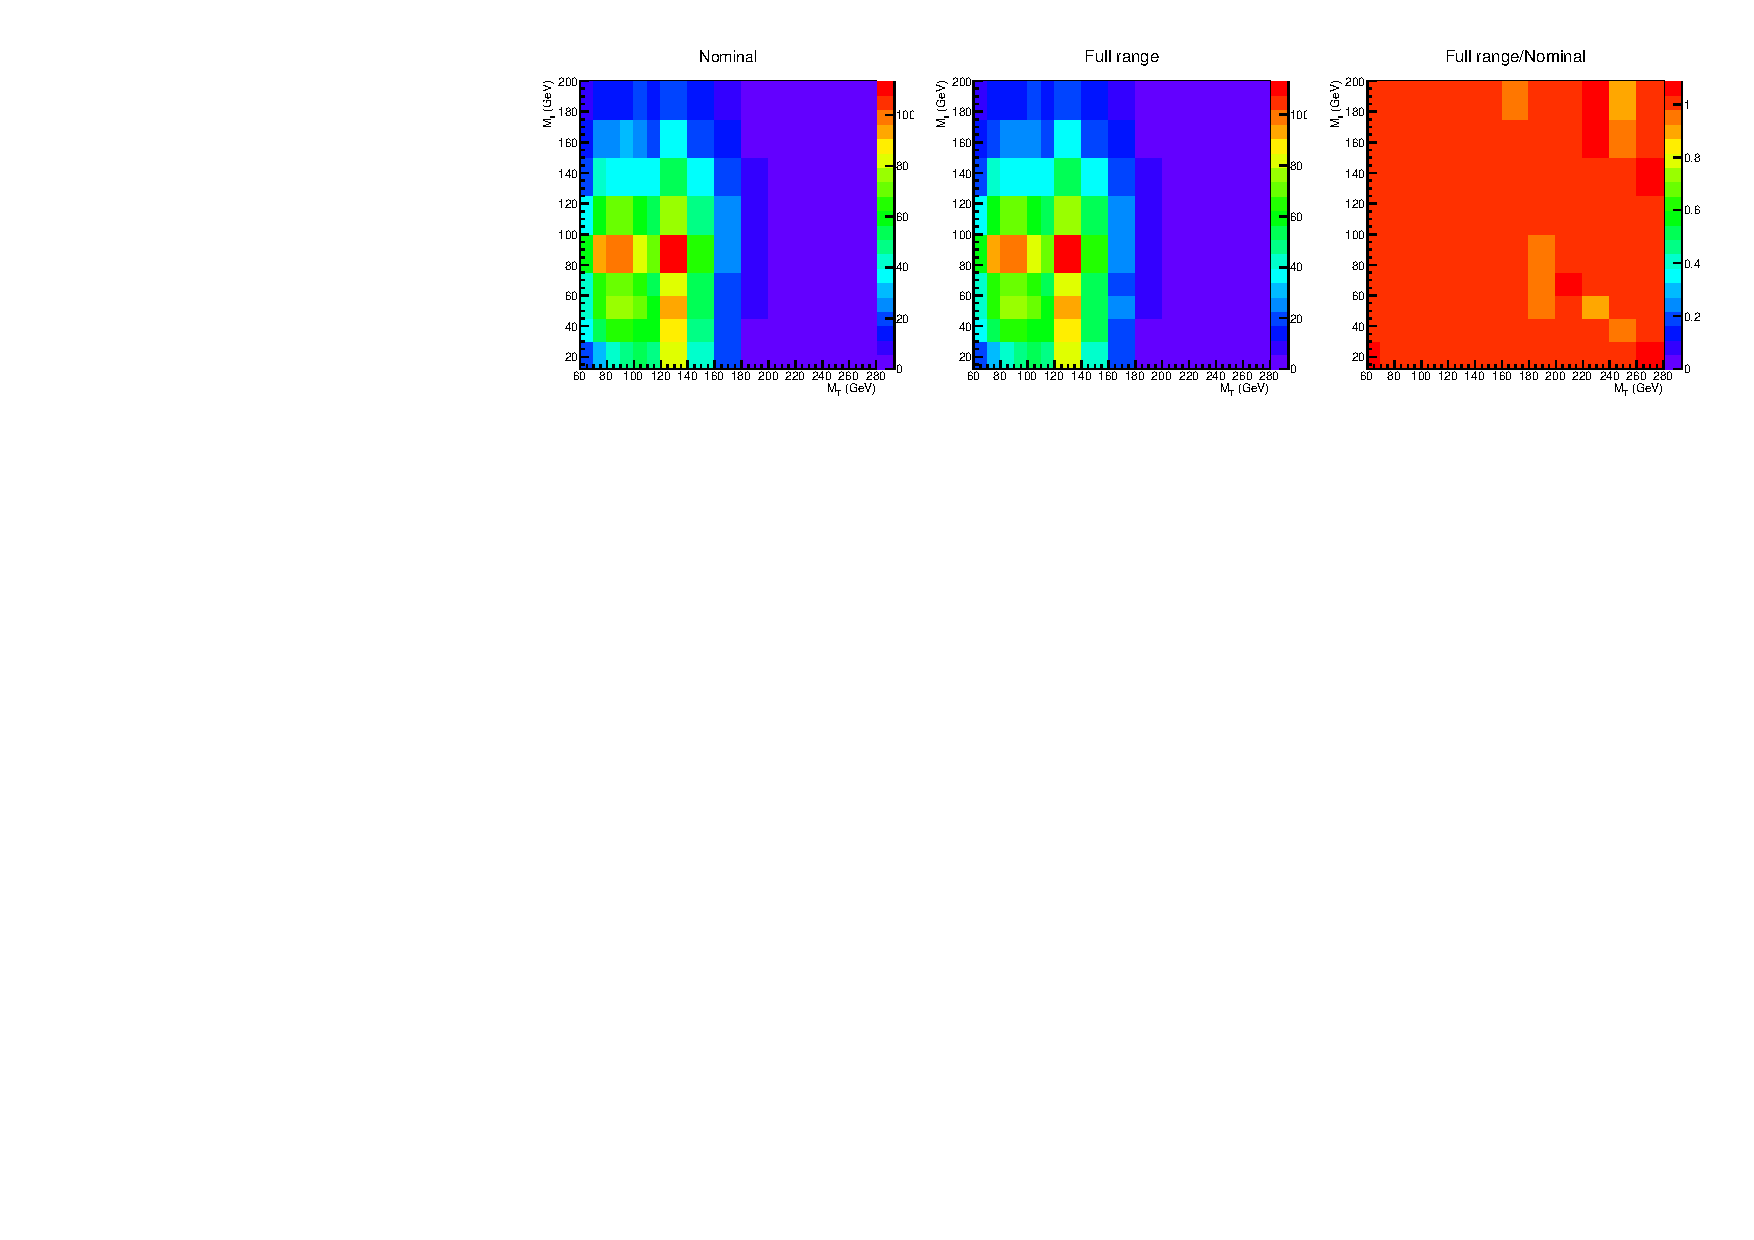
\includegraphics[width=1.0\textwidth]{figures/2Dshape_sanity.pdf}
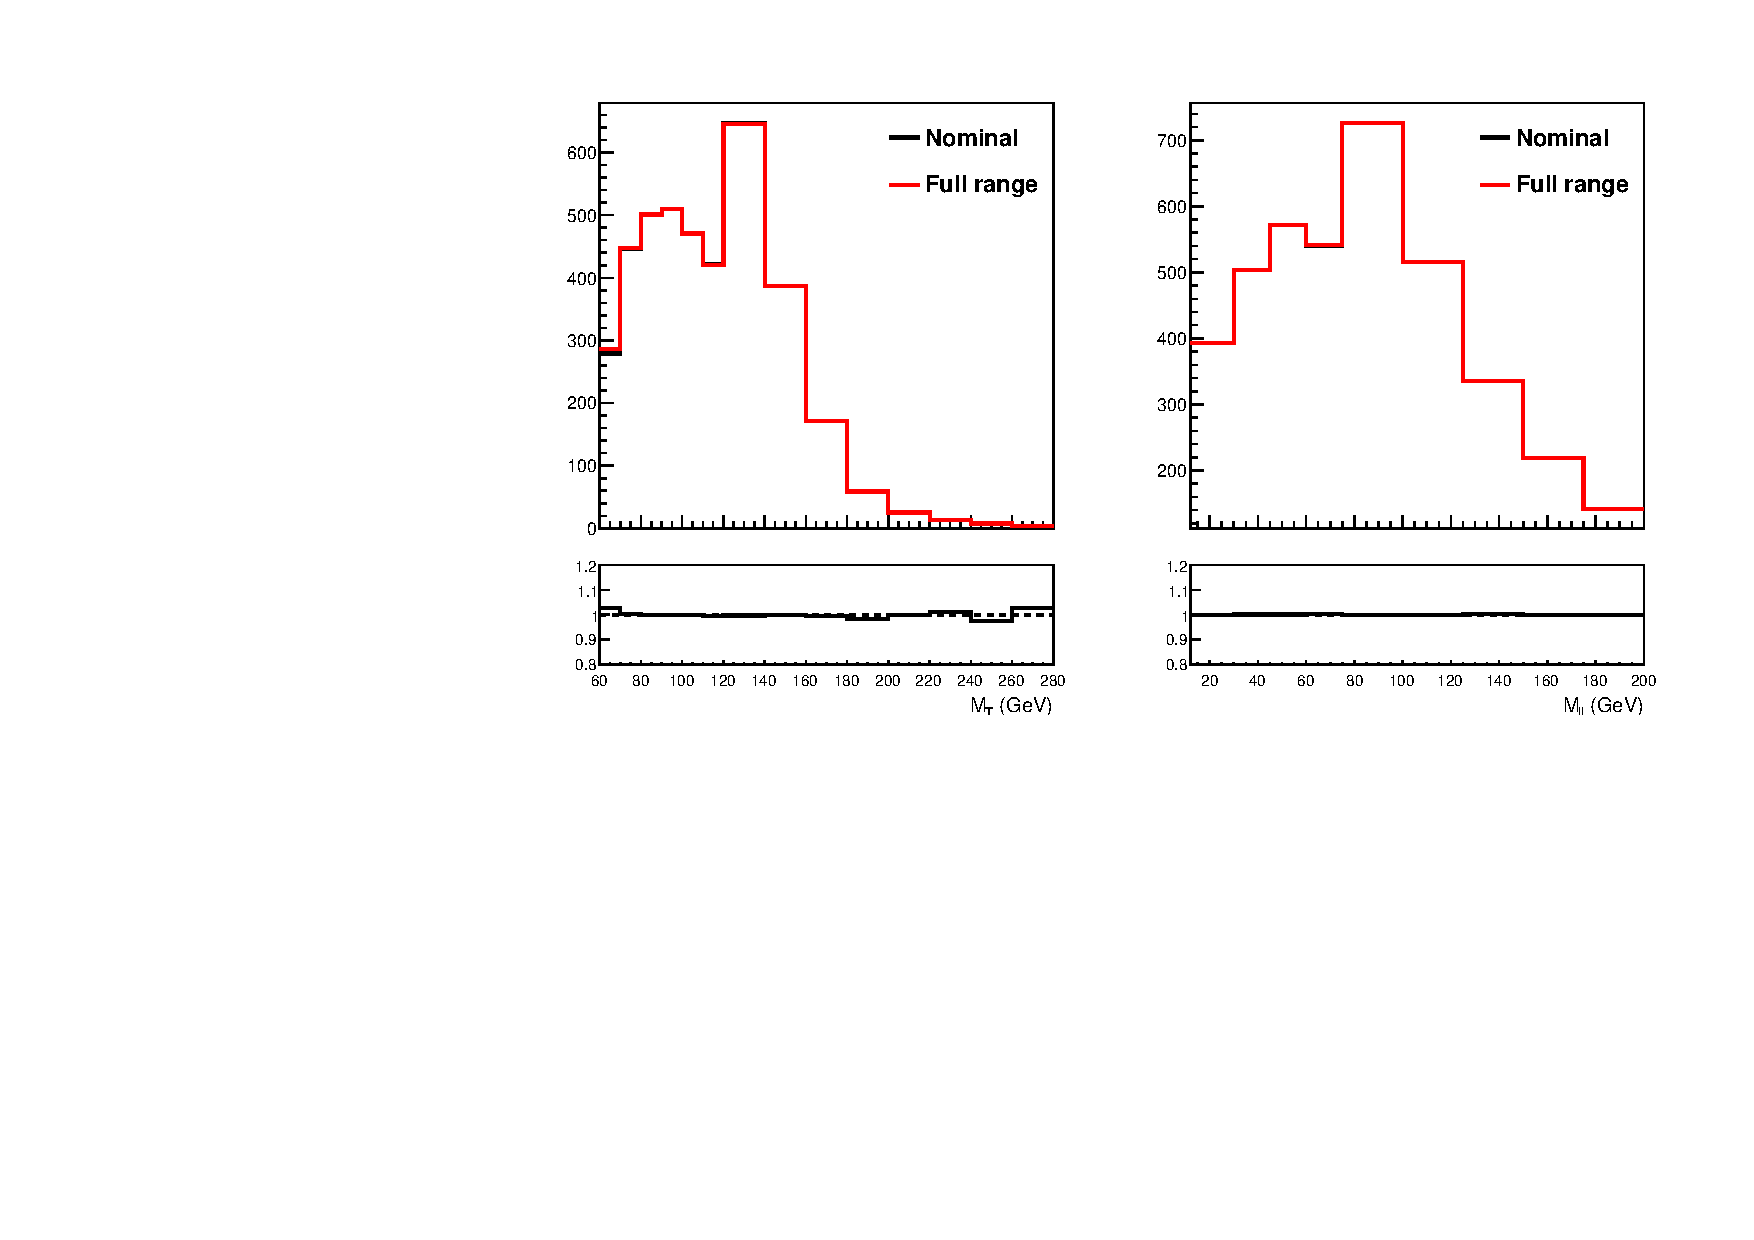
\includegraphics[width=0.8\textwidth]{figures/1Dshape_sanity.pdf} 
\caption{Comparison of post-fit shapes from nominal and full range fits.}
\label{fig:sanity_fullrange}
\end{figure}
%
\begin{table}
\begin{center}
\begin{tabular}{c|cccc}
\hline
Fit         & \qqVH    & \qqH   & \ggH   & \qqww          \\
\hline
Nominal     & 4.8   & 1.9   & 144.3 &  3945.4       \\
Full range  & 4.8   & 1.9   & 143.6 &  3947.0       \\
\hline
\end{tabular}
\end{center}
\caption{Comparison of normalization from nominal and full range fits.} 
\label{tab:sanity_fullrange}
\end{table}
As a sanity check we compare the post-fit shape and normalization of \qqww\
from the full range fit with those from the nominal fit in 
Figure~\ref{fig:sanity_fullrange} and Table~\ref{tab:sanity_fullrange}. 
Both shapes and normalizations using full range card 
are consistent with the nominal fit results. 

Since the full range fit has been validated, 
we perform two fits using only one of the control regions.
The fit using CR1(2) will be denoted as CR1(2) fit hereafter. 
In a fit using one control region, 
the other region is removed in the fit, and the normalization of each process 
is fixed accordingly. 

\begin{figure}[!hbtp]
\centering
\subfigure[\mll\ in CR1]{
\centering
\label{subfig:cr1_mll}
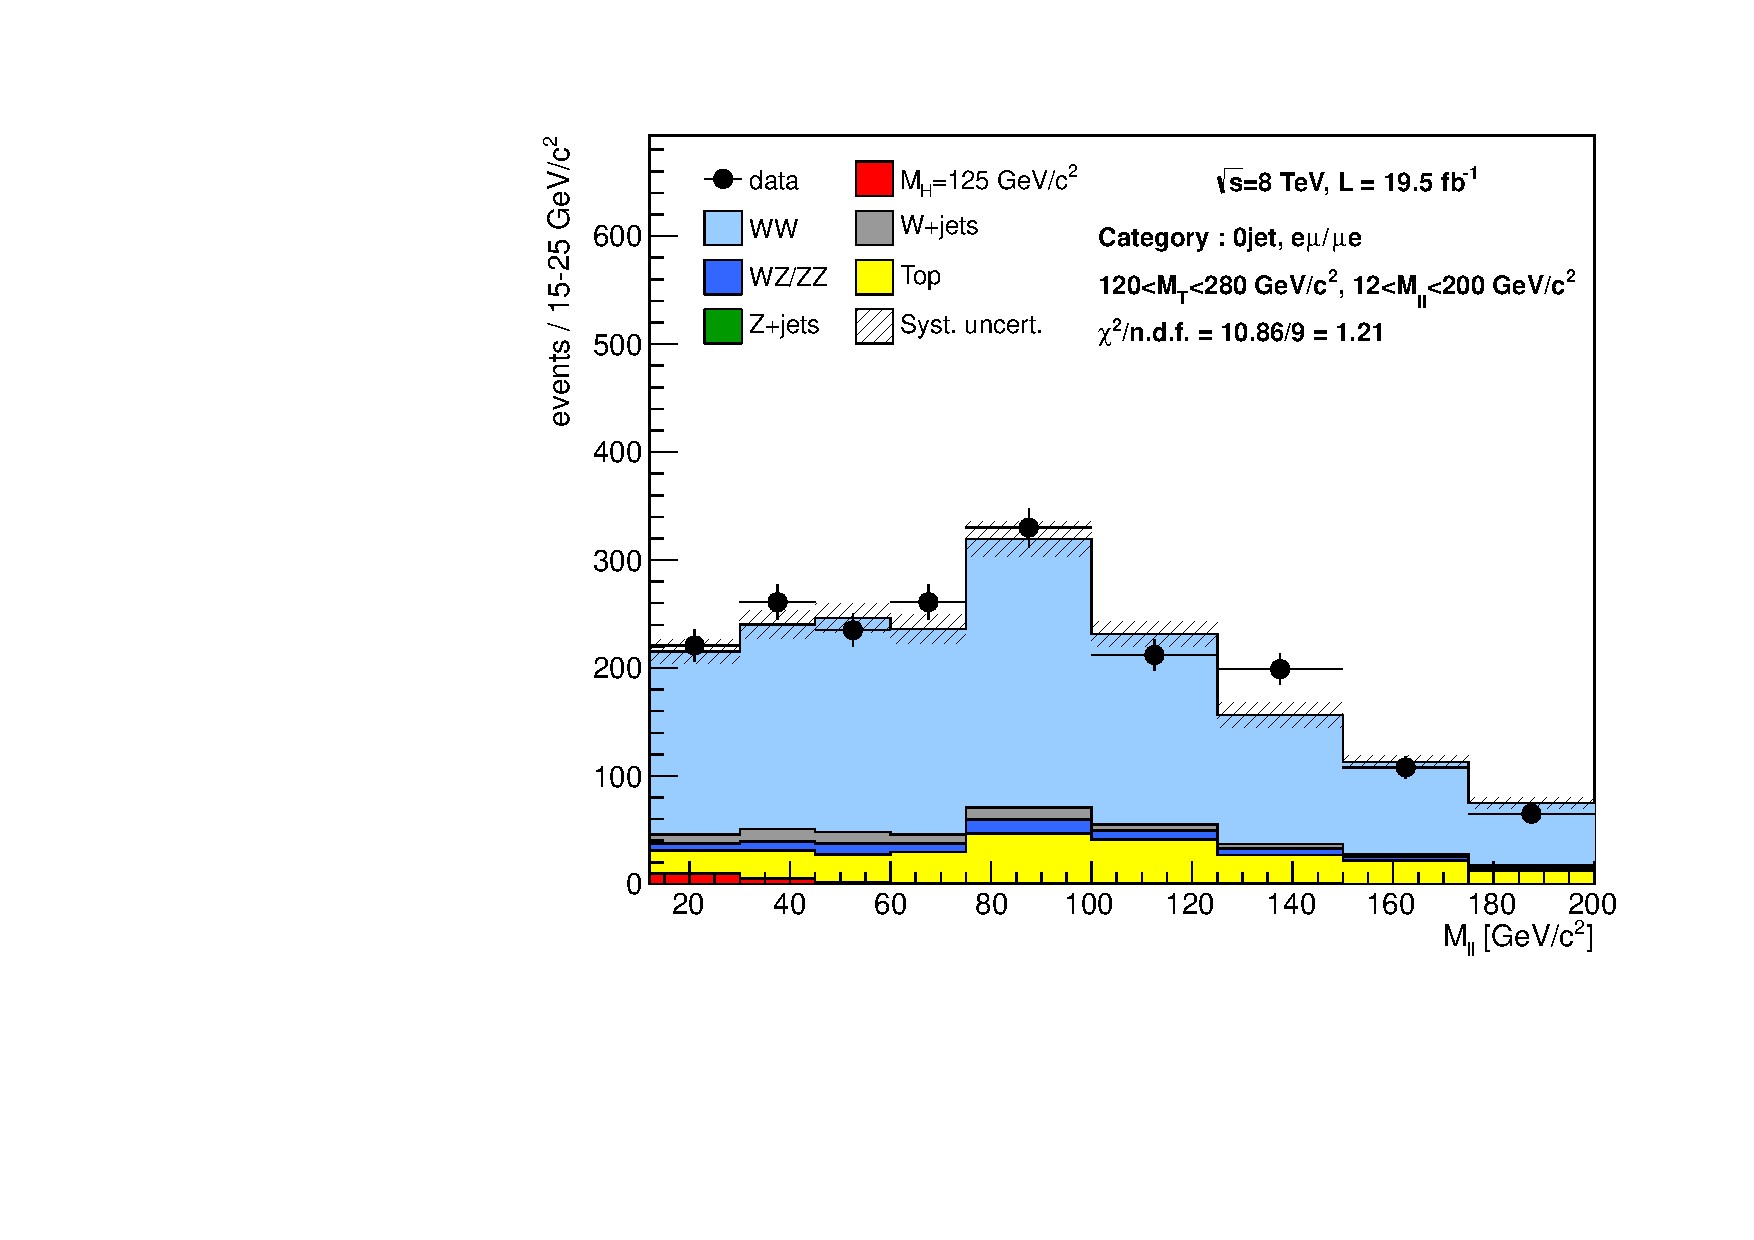
\includegraphics[width=.47\textwidth]{figures/mll_CR1.pdf}
}
\subfigure[\mT\ in CR1]{
\centering
\label{subfig:cr1_mT}
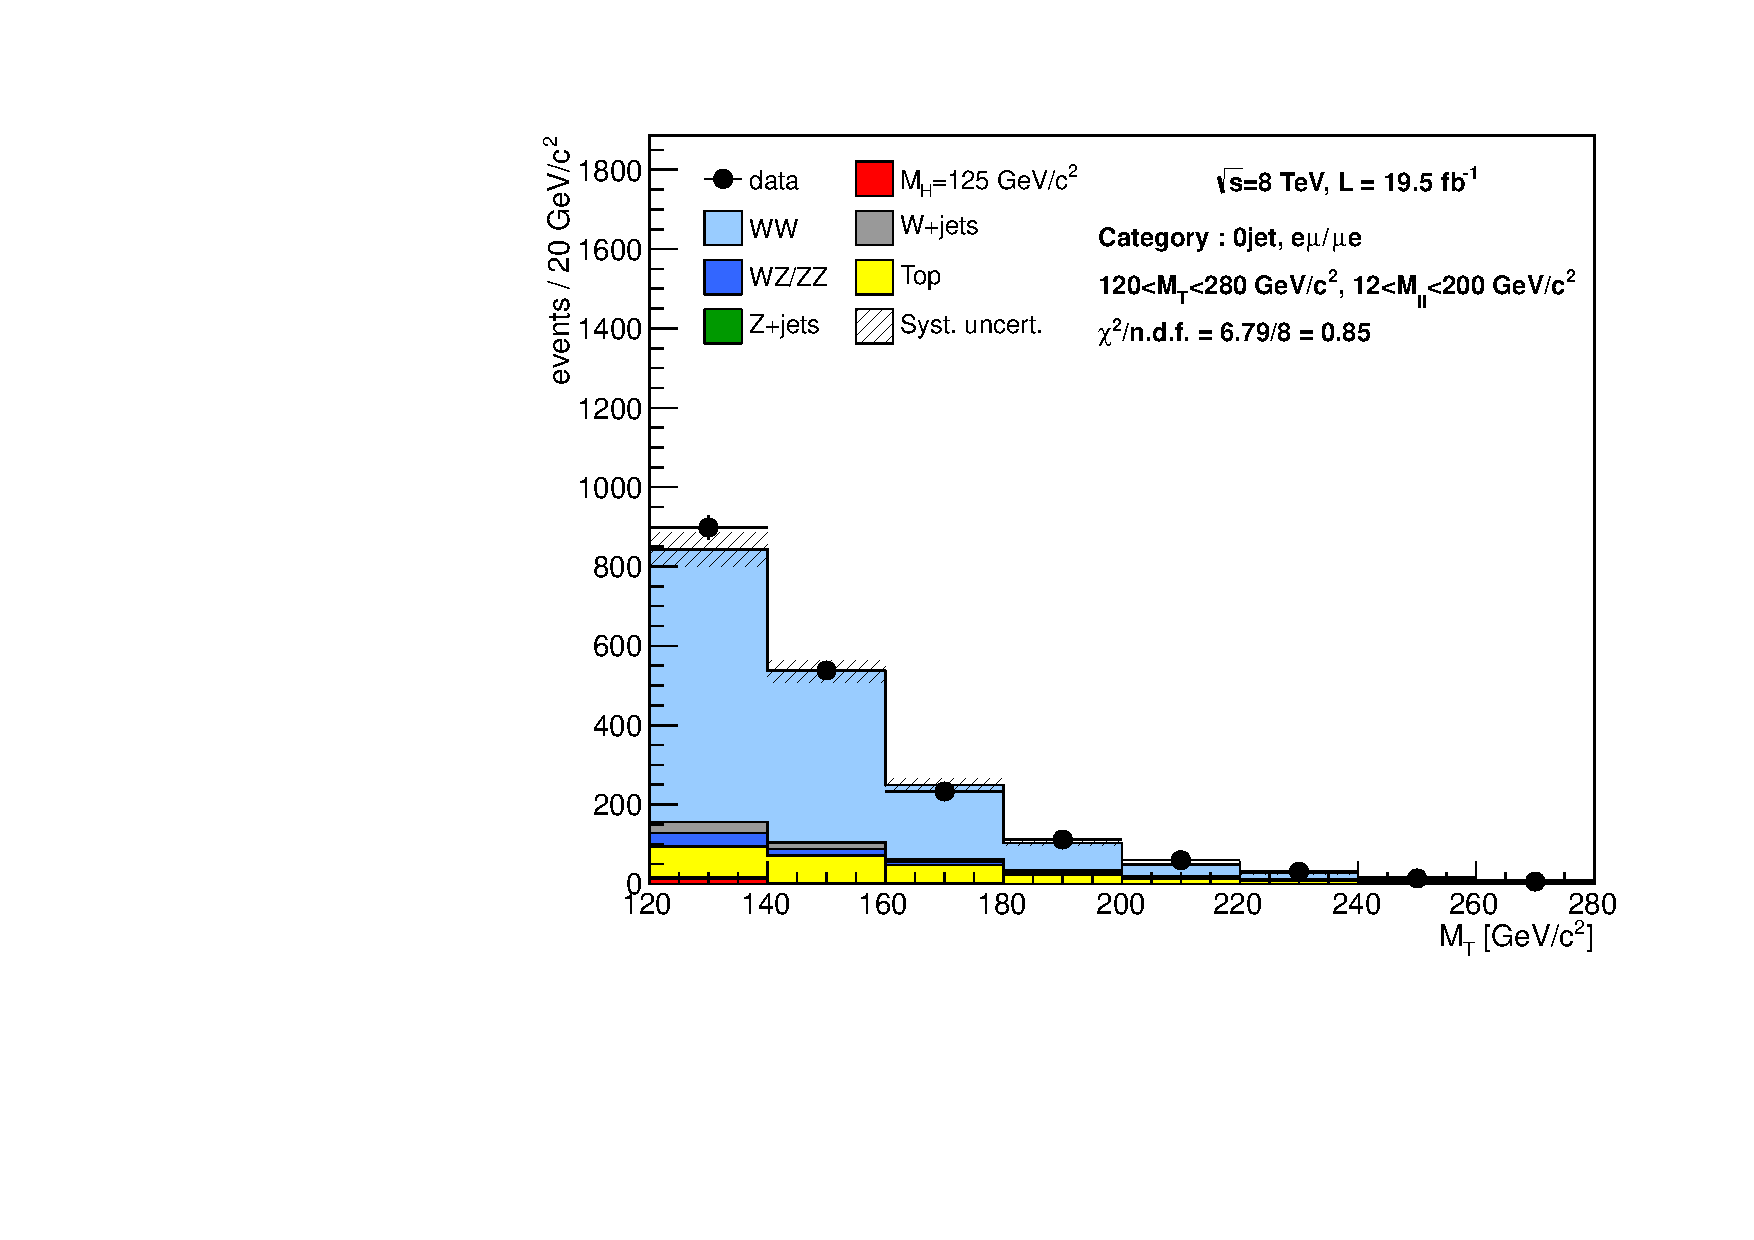
\includegraphics[width=.47\textwidth]{figures/mT_CR1.pdf}
}\\
\subfigure[\mll\ in CR2]{
\centering
\label{subfig:cr2_mll}
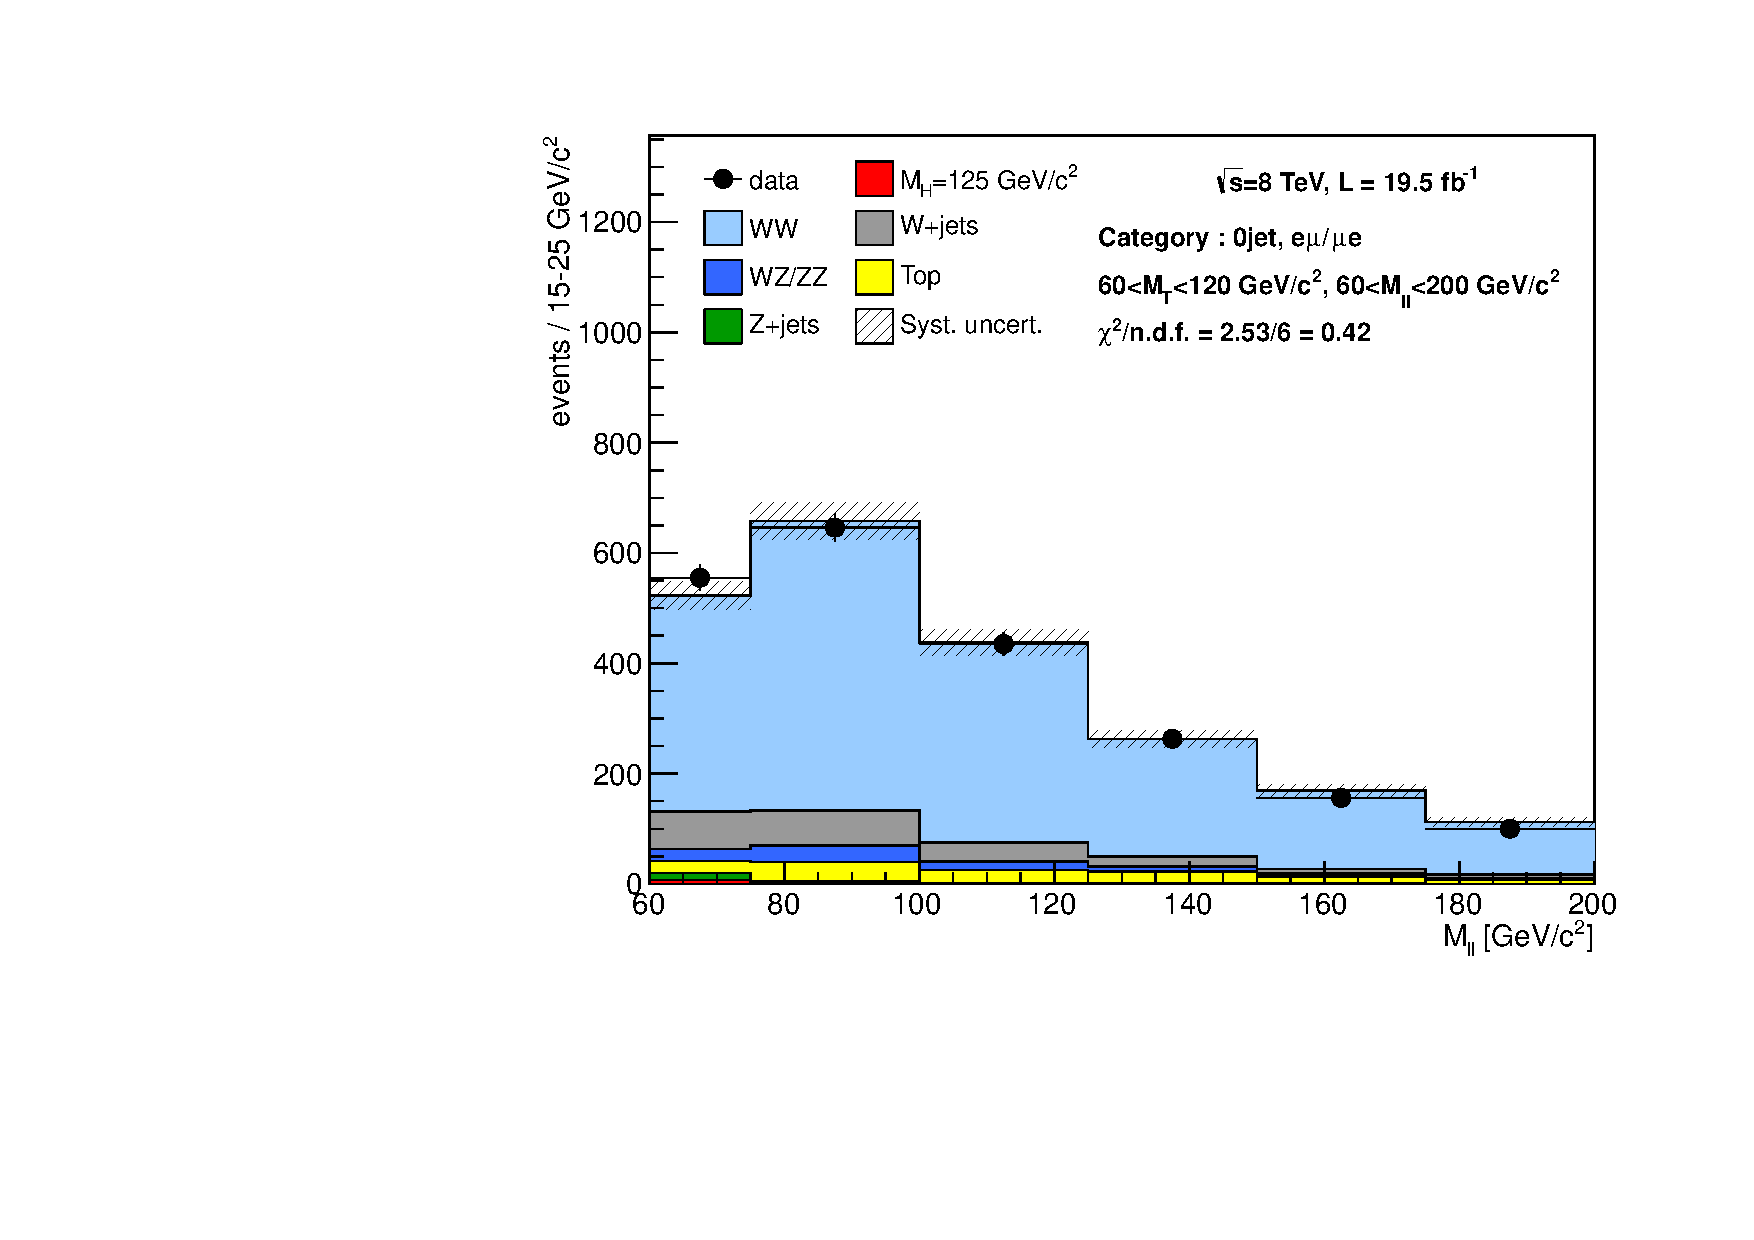
\includegraphics[width=.47\textwidth]{figures/mll_CR2.pdf}
}
\subfigure[\mT\ in CR2]{
\centering
\label{subfig:cr2_mT}
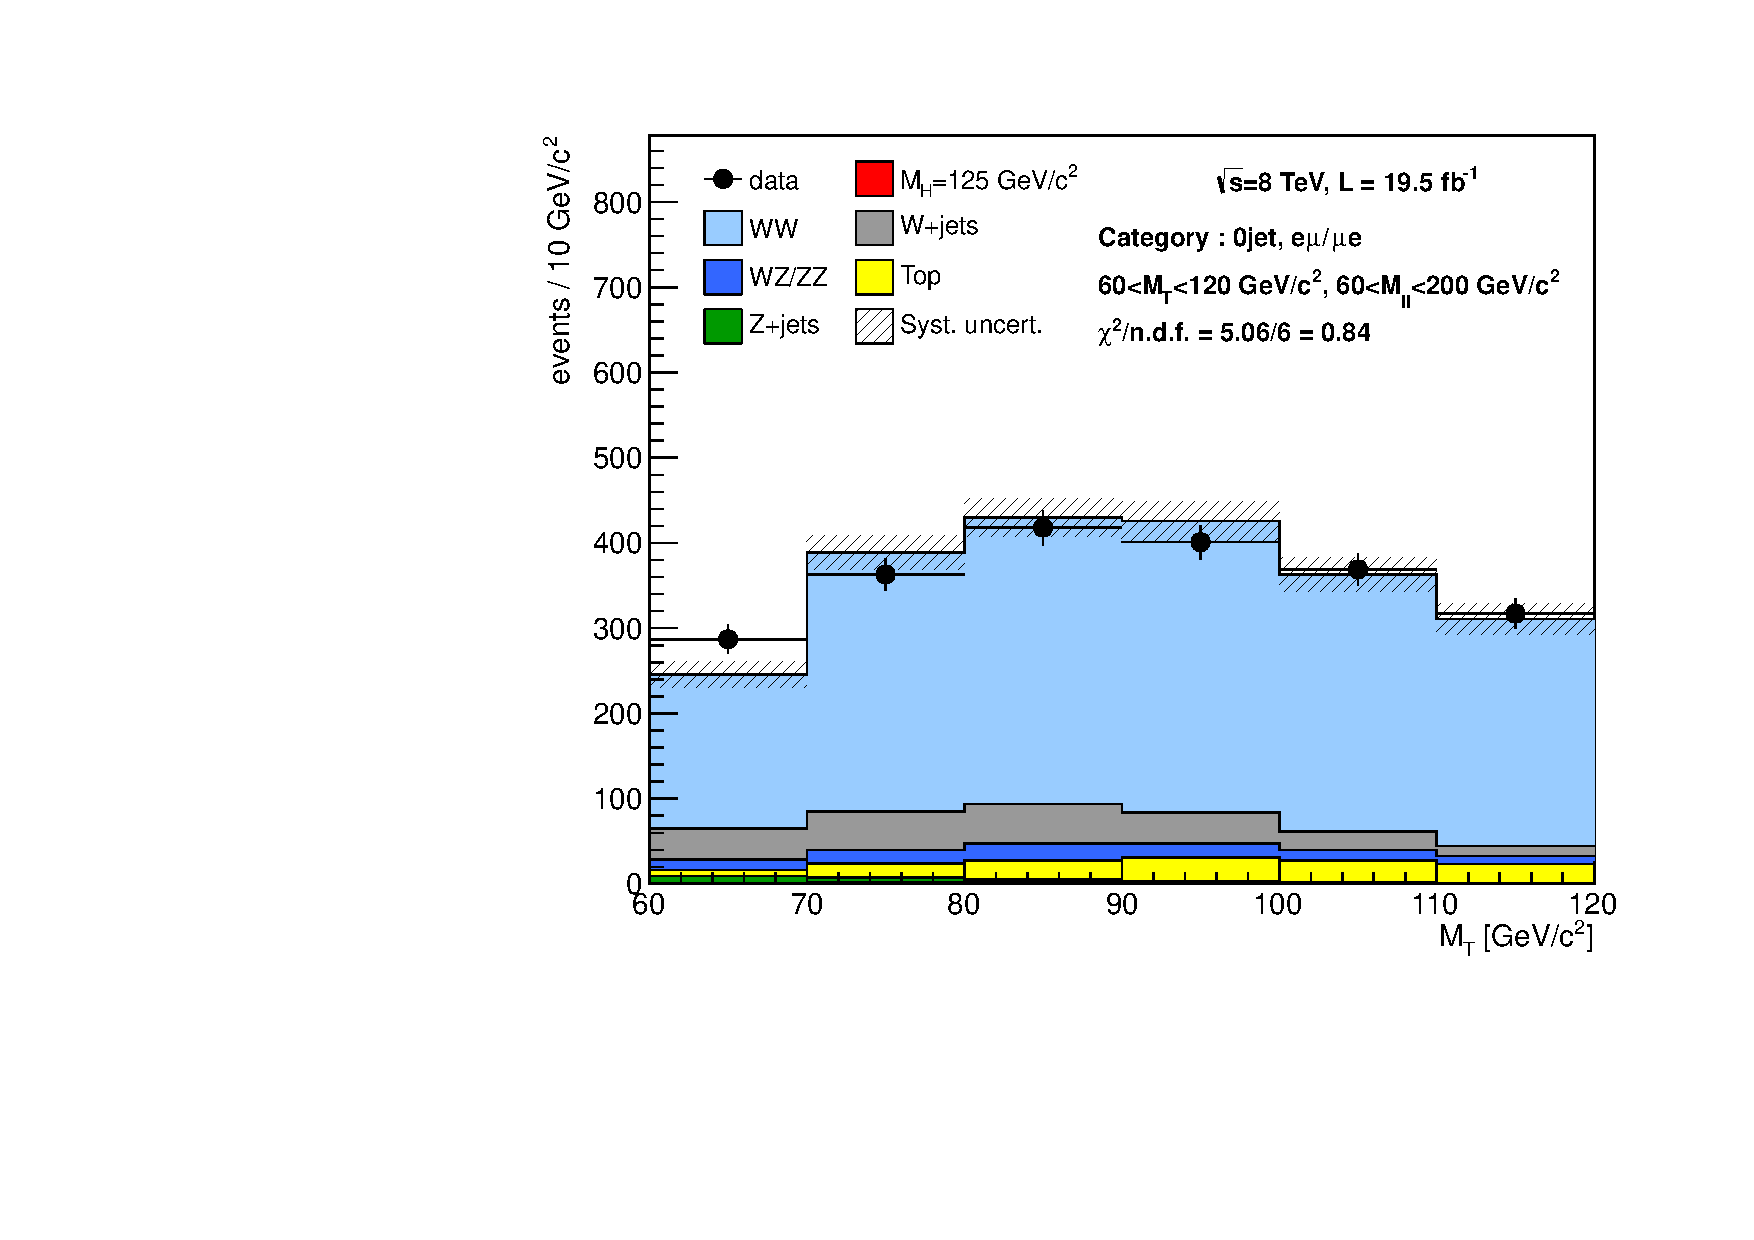
\includegraphics[width=.47\textwidth]{figures/mT_CR2.pdf}
}\\
\caption{\mll(a,c) and \mT(b,d) distributions in CR1(top) and CR2(bottom) 
using the fit results of CR2 and CR1.}
\label{fig:wwctl_final}
\end{figure}

Figure \ref{fig:wwctl_final} shows the \mT\ and \mll\ distributions in CR1 and CR2 using 
the post-fit result from the other control regions. 
The uncertainty band is the post-fit uncertainty obtained by pseudo-data sets 
generated using the post-fit uncertainties. 
The variances in each bin of \qqww\ and all other backgrounds 
are taken from the full range and the nominal fits, respectively, 
and are added in quadrature. 
The agreement between data and prediction is measured by
\begin{equation} 
\chi^2/n.d.f.
= \frac{1}{N_{bin}} \displaystyle \sum_{i=1}^{N_{bin}}  
  \frac{\left( N^{data}_i - N^{simulation}_i \right)^2}
       {\left( \sigma^{data}_i \right)^2 + \left( \sigma^{simulation}_i \right)^2}   
\end{equation}  
where $N_{bin}$ is the number of bins, 
$N^{data(simulation)}_i$ is the yield of data(simulation) in the $i^{th}$ bin
and $\sigma^{data(simulation)}_i$ is the uncertainty of data(simulation) 
in the $i^{th}$ bin. As shown on each plot, the $\chi^2/n.d.f.$
is close to 1, which means that all distributions show a good agreement with data.

This indicates that our \qqww\ fit model is not biased.
%
\begin{table}
\begin{center}
\begin{tabular}{c|ccc}
\hline
                    & full range fit    & CR1 fit   & CR2 fit   \\
\hline \hline
Best-fit $\mu$      & 0.63              & 0.63      & 0.62      \\
\hline
\end{tabular}
\end{center}
\caption{Comparison of the best-fit $\mu$ values from the full range, CR1 and CR2 fits.} 
\label{tab:bestfitmu_compare}
\end{table}

Table~\ref{tab:bestfitmu_compare} shows the best-fit $\mu$ values from full range, 
CR1 and CR2 fits. Using different control regions results in consistent 
best-fit $\mu$ values. 
This is an another evidence that our fit model is correct. 

Therefore, we conclude that our fit model for \qqww\ process fits data correctly.  

%%%%
\subsection{Validation of \topbkg\ fit model} 

By inverting the top-tagging requirement, we can select an event sample 
dominated by \topbkg\ events. We perform the same shape-based analysis 
with templates constructed using the top-tagged events. 
The Figure~\ref{fig:topCRfit} shows the \mll\ and \mT\ distributions 
after normalizing the shape to the post-fit result. The agreement 
between the post-fit fit result and data is good, and we conclude 
that the \topbkg\ fit model is correct. 

\begin{figure}[!hbtp] 
\begin{center}
    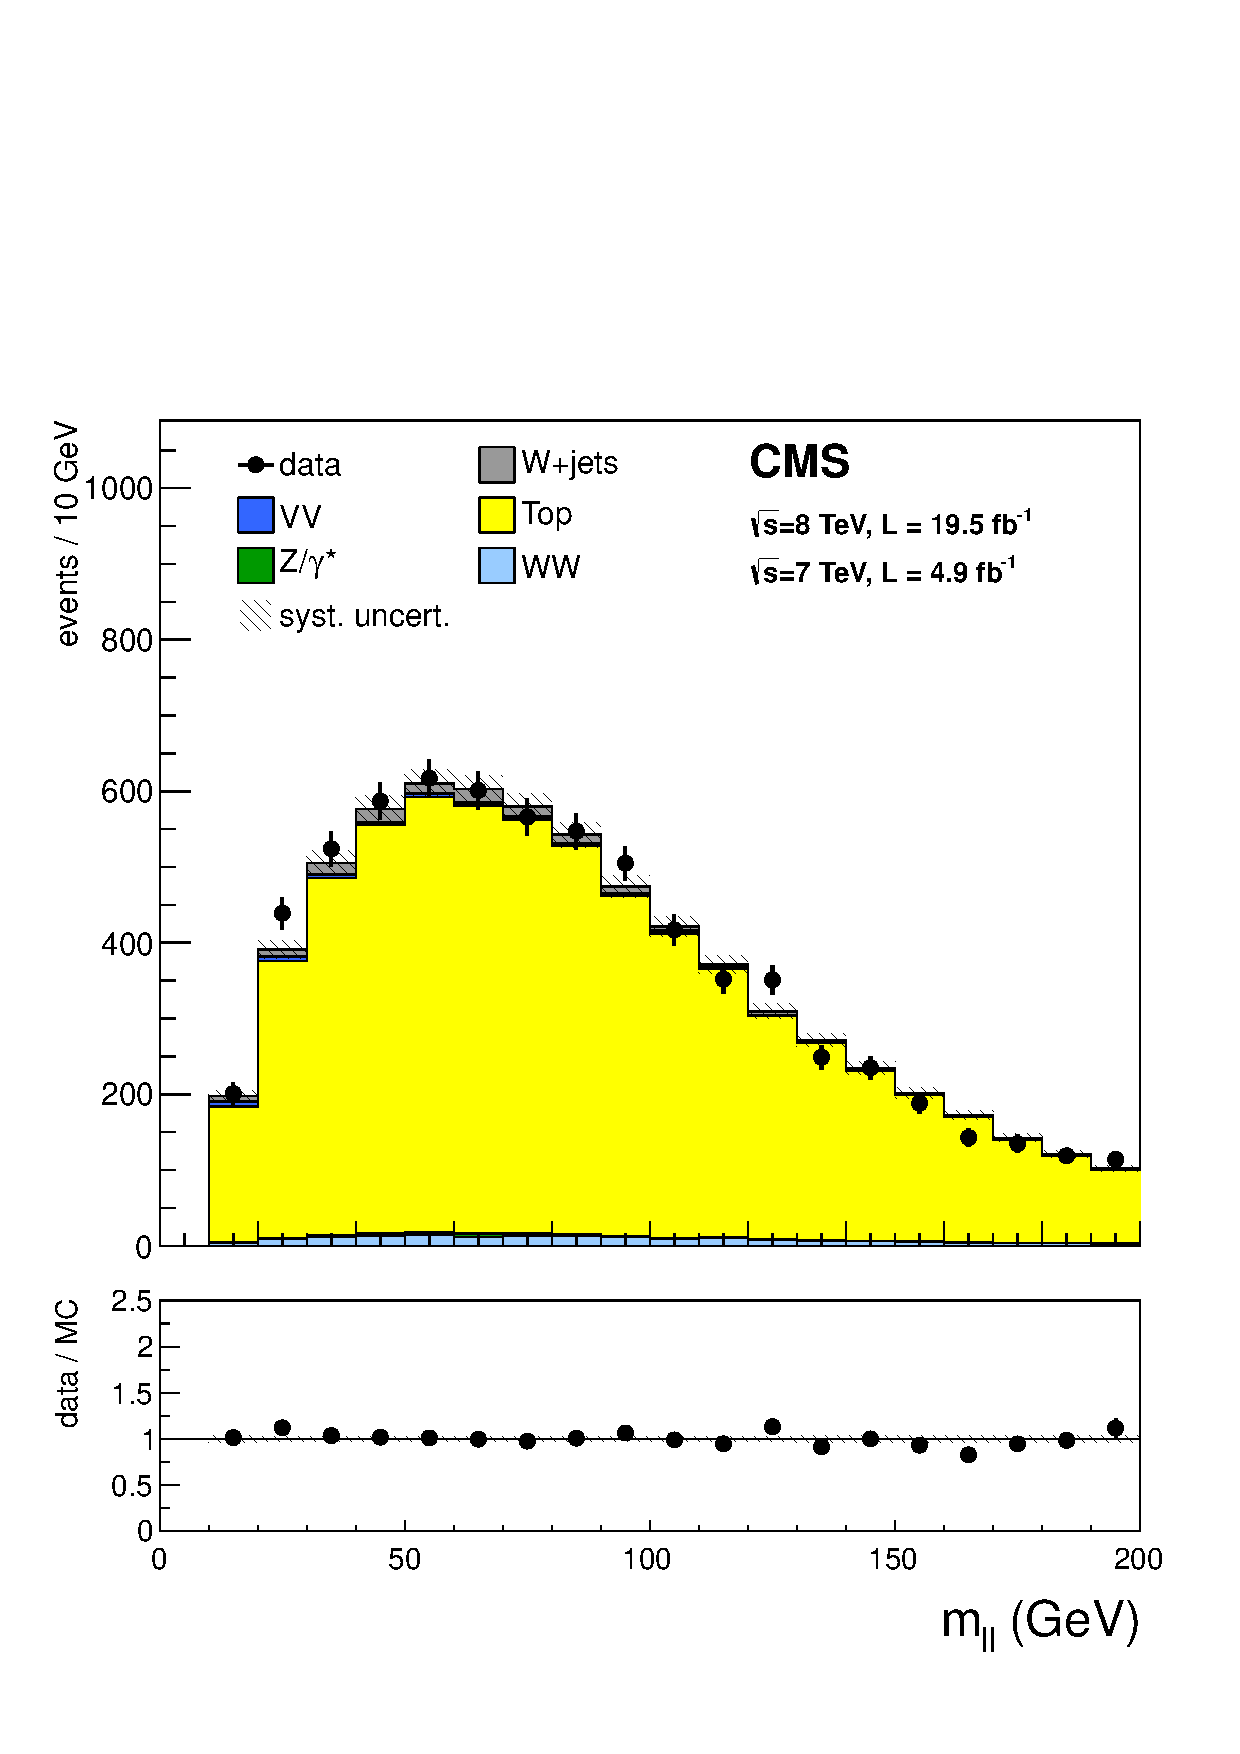
\includegraphics[width=.47\textwidth]{figures/Top_mll_1j.pdf}
    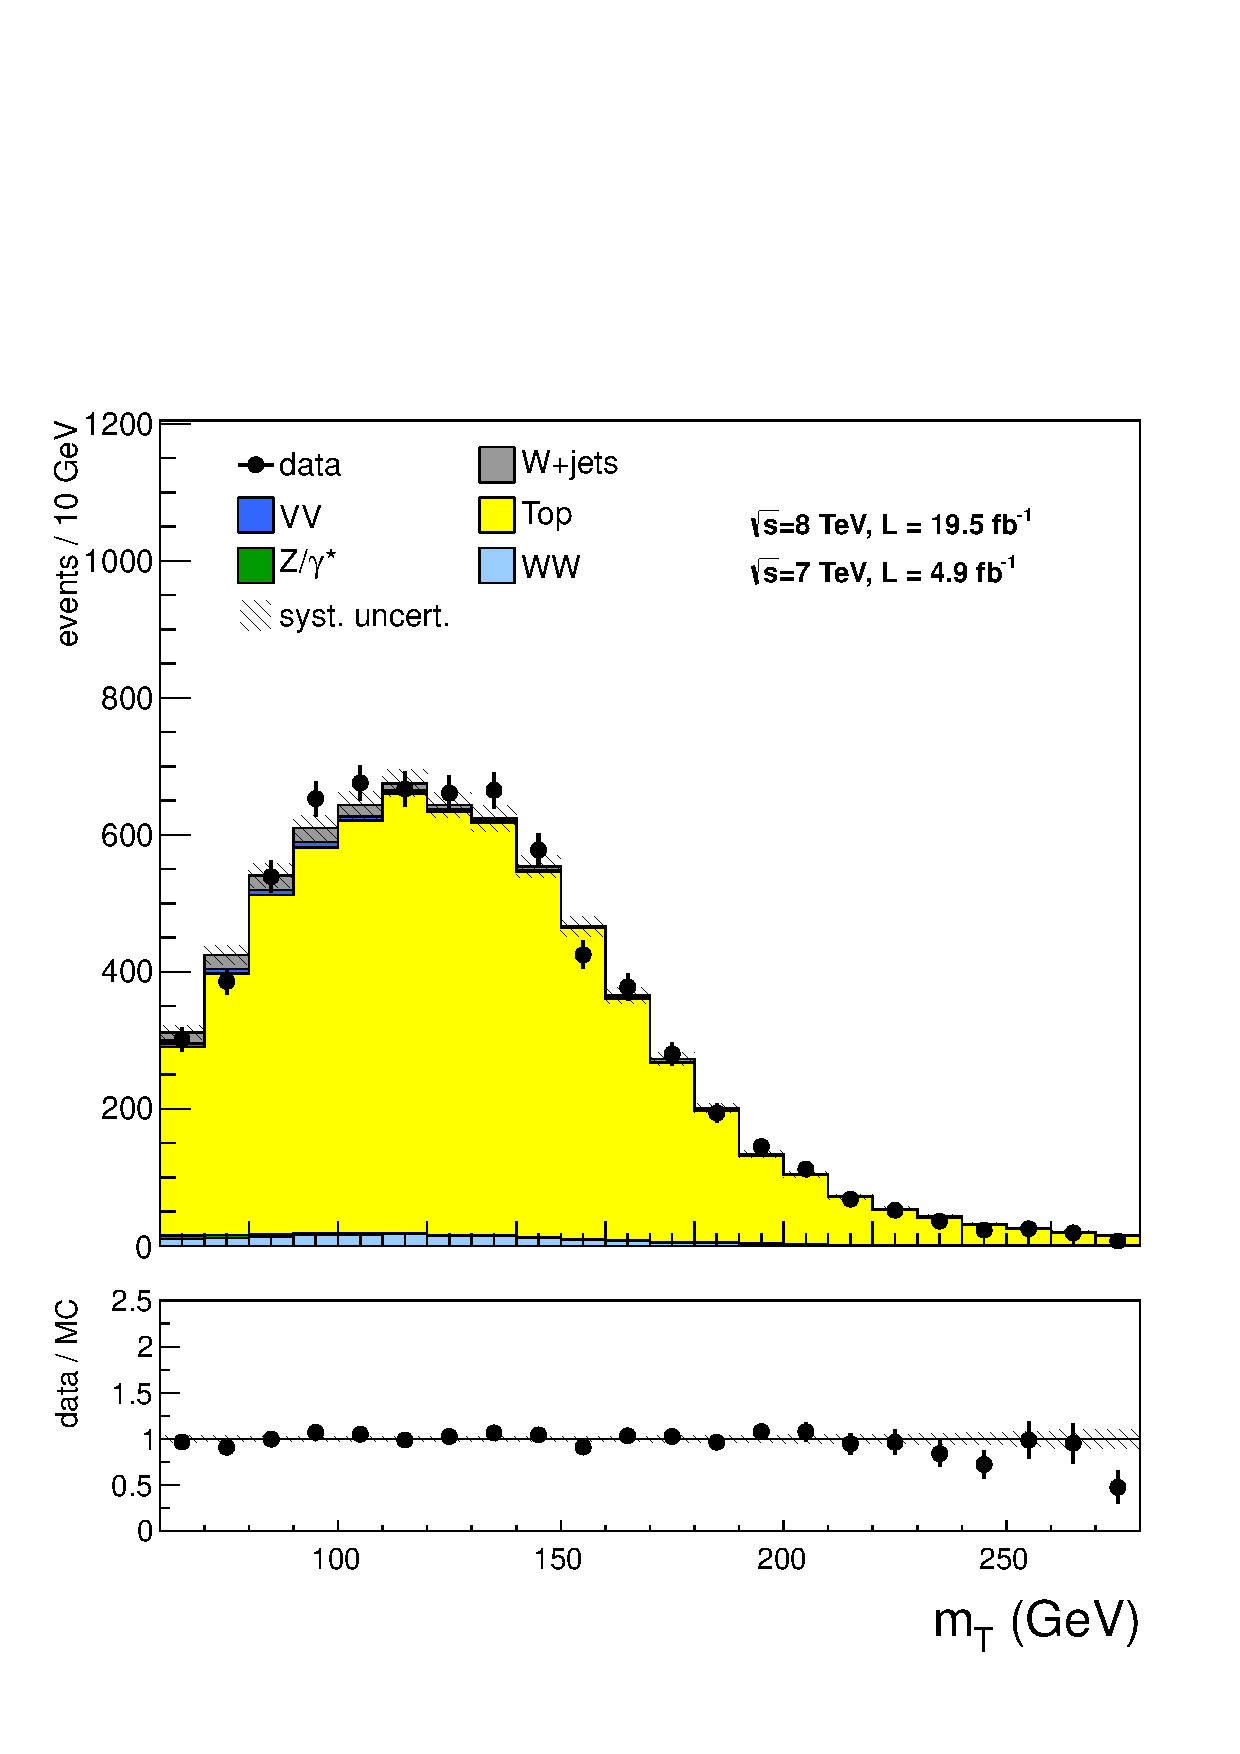
\includegraphics[width=.47\textwidth]{figures/Top_mT_1j.pdf}
    \caption{The post-fit \mll\ and \mT\ distributions in the top-tagged region.} 
    \label{fig:topCRfit}
\end{center}
\end{figure}


%%%%
\subsection{Validation of \Wjets\ and \wgamma/\wgammastar\ fit models}  

By inverting the opposite-sign requirement on the leptons, 
we can select an event sample dominated by \Wjets\ and \wgamma/\wgammastar\ events. 
We perform the same shape-based analysis
with templates constructed using the same-sign events.
The Figure~\ref{fig:ssCRfit} shows the \mll\ and \mT\ distributions
after normalizing the shape to the post-fit result. The agreement
between the post-fit fit result and data is good, and we conclude
that the \Wjets\ and \wgamma/\wgammastar\ fit models are correct.

\begin{figure}[!hbtp] 
\begin{center}
    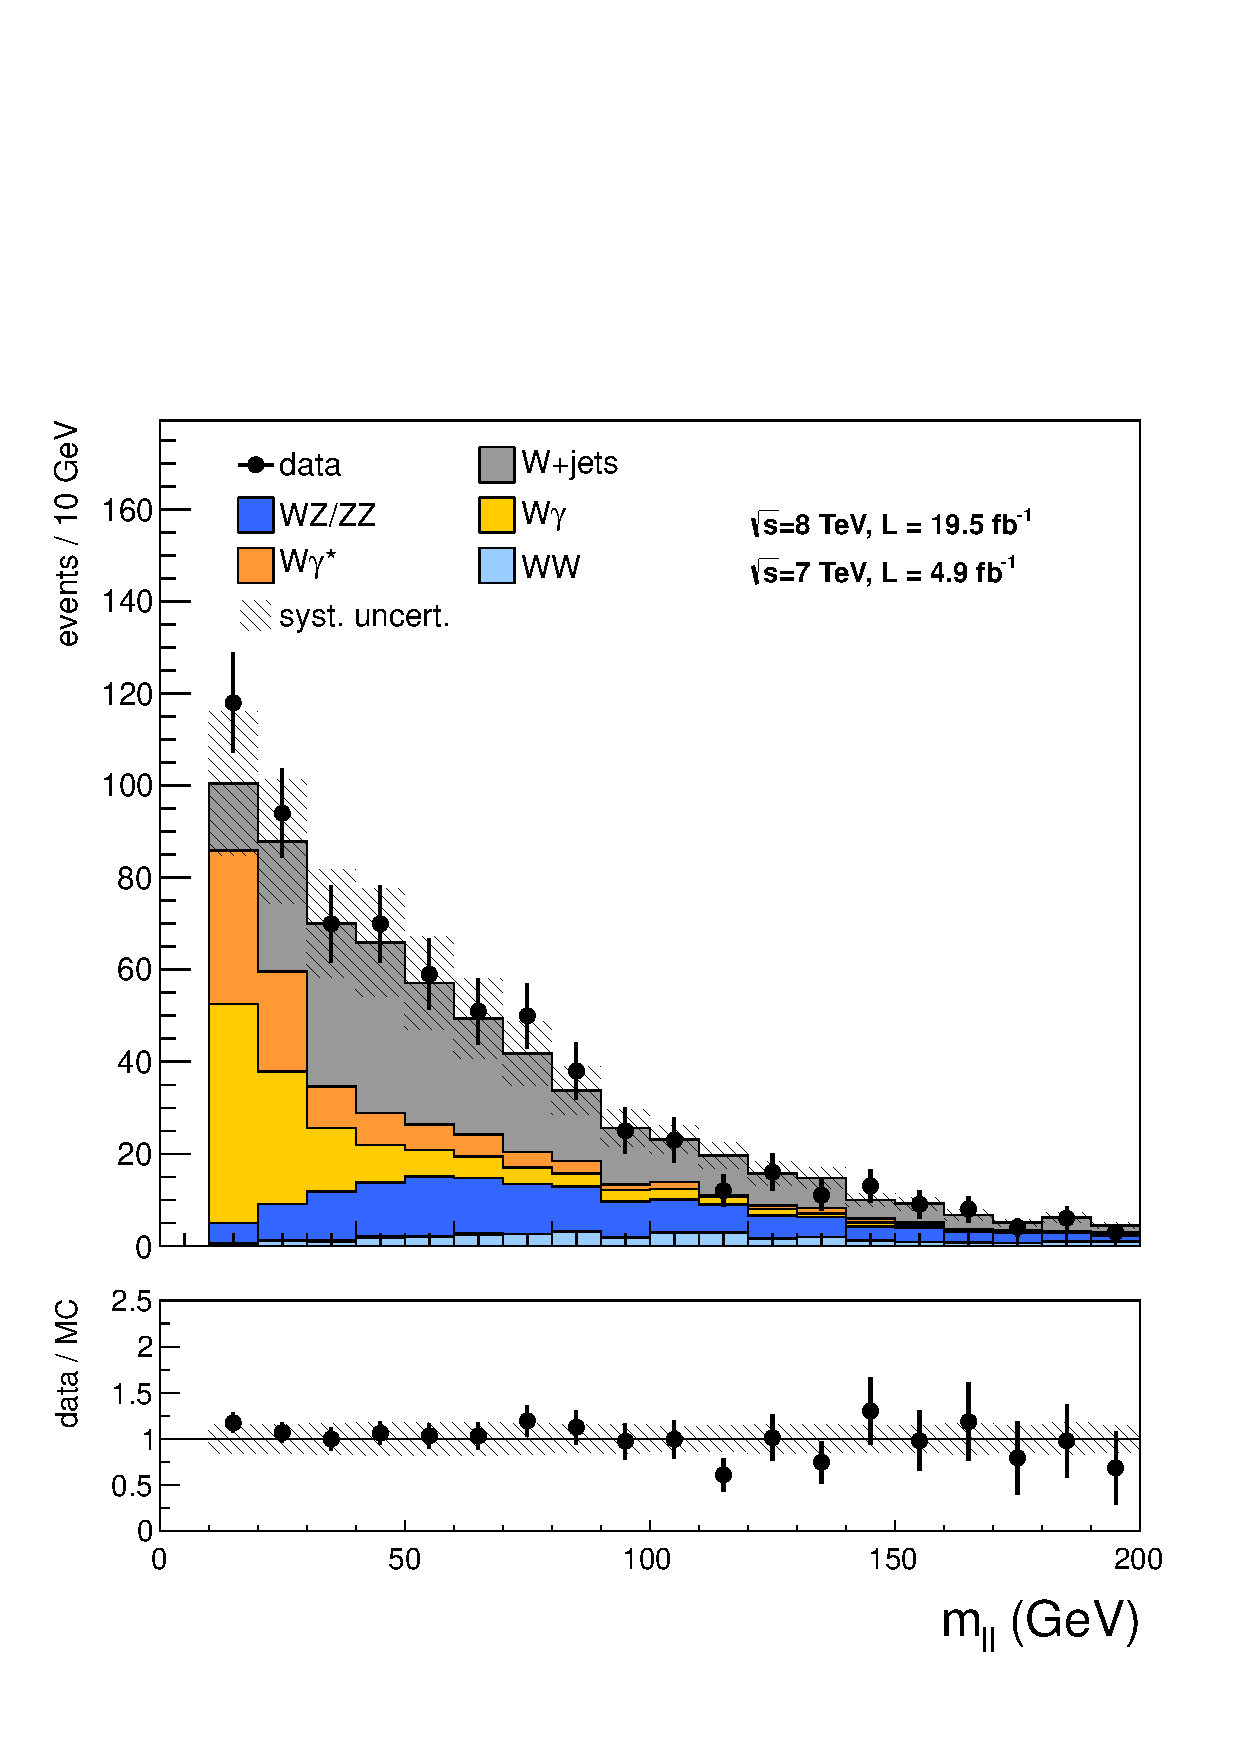
\includegraphics[width=.47\textwidth]{figures/SS_mll_0j.pdf}
    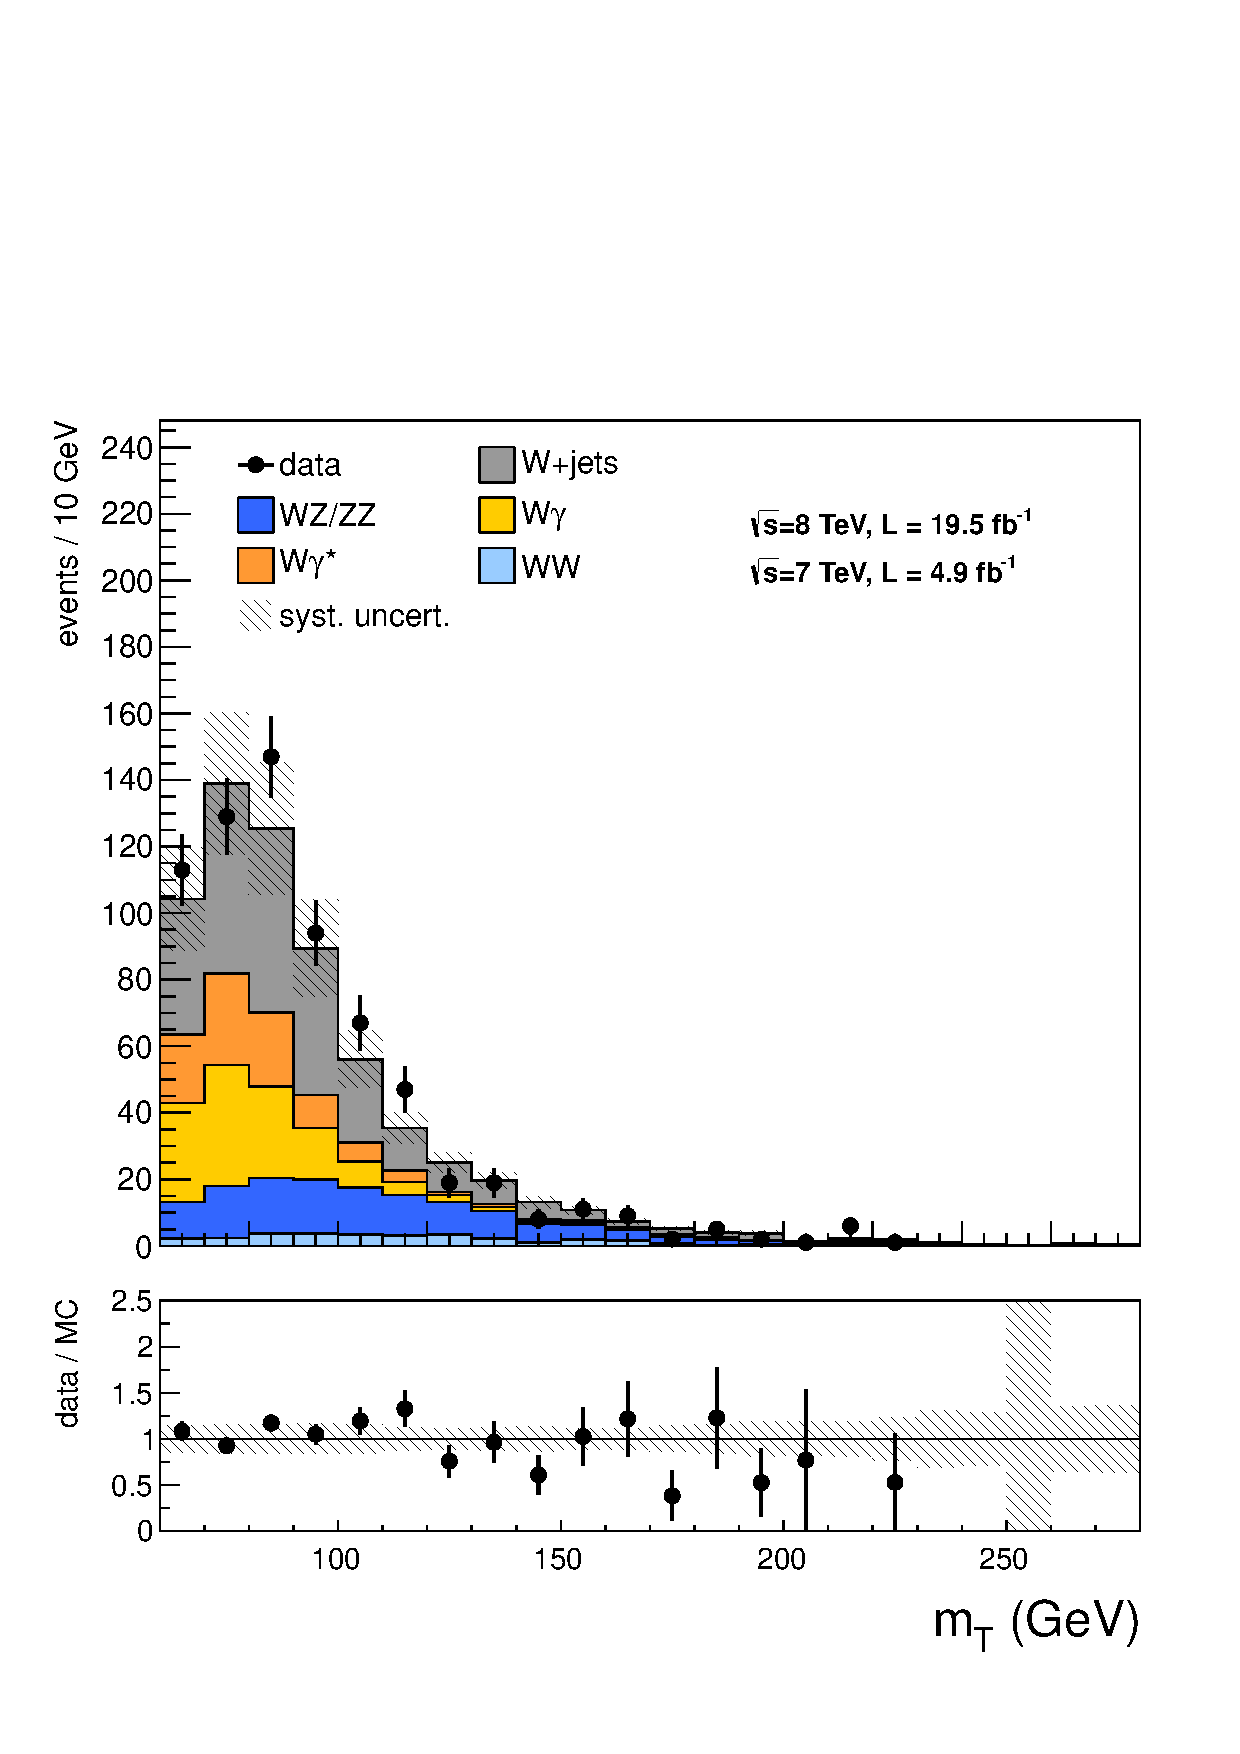
\includegraphics[width=.47\textwidth]{figures/SS_mT_0j.pdf}
    \caption{The post-fit \mll\ and \mT\ distributions in the same-sign region.} 
    \label{fig:ssCRfit}
\end{center}
\end{figure}



%%%%%%%%%%%%%%%%%%%%%%%%%%%%%%%%%%%%%%%%%
\section{Post-fit Analysis}

Fit is a tool that determines the normalization and shape of the 
signal and the backgrounds that describes the data best. 
We use the maximum likelihood fit that scans nuisances, and finds 
the point where the likelihood has its maximum. The tool 
can do what is best in terms of finding the maximum, but 
sometimes the result does not make sense, which might 
indicate that our fit model is not correct. 

This section thus discusses the post-fit result of the fit 
to confirm that the fit is stable, and the result makes sense. 

\subsection{Post-fit result of nuisances}

In an ideal world where prediction of the central value of a nuisances is 
exactly what nature gives, the nuisance should not change by fit. But, in reality 
prediction can be wrong, thus we assign uncertainty on the nuisances. On the other 
hand, if the prediction is wrong by a large margin, the post-fit value of the nuisance 
can be far from the prediction, even larger than the uncertainty we assign. 
So, we need to make sure that the post-fit nuisances are within the assigned uncertainty.
A large variation of nuisances may indicate that the fit model does not 
describe data correctly. 

The measure to check this is the ``Pull" which is defined as 
\begin{eqnarray} 
\textrm{Pull} = \frac{\theta_{\textrm{post-fit}} - \theta_{\textrm{pre-fit}}}{\sigma_{\textrm{pre-fit}}}  
\end{eqnarray} 
where $\theta_{\textrm{pre-fit(post-fit)}}$ is the central value of a nuisance 
before(after) the fit, and $\sigma_{\textrm{pre-fit}}$ is the assigned uncertainty 
to that nuisance. If the prediction is perfect, and there is no variation of 
the nuisance by fit, then the Pull should be 0. The Pull with larger than 1, 
\textit{i.e.} the variation if larger than the assigned error, may indicate 
that the fit model is not correct or a lack of understanding of that nuisance. 

One of the reasons why we rely on fit is that the data can constrain nuisances 
more than the assigned uncertainties. If there is a region that is dominated by 
a certain background process then the fit can use that region to constrain that 
background. But, if the post-fit uncertainty is larger than the assigned one, 
this might be an evidence that the assigned uncertainty is smaller than what is 
supposed to be. In order to assess any effects of this kind, we define the 
normalized uncertainty, $\sigma_{\textrm{norm}}$, which is defined as a 
ratio of the post-fit uncertainty to the pre-fit uncertainty of a nuisance, 
\begin{eqnarray} 
\sigma_{\textrm{norm}} = \frac{\sigma_{\textrm{post-fit}}}{\sigma_{\textrm{pre-fit}}}. 
\end{eqnarray} 
The $\sigma_{\textrm{norm}}$ larger than 1 means that the nuisance is not constrained by 
fit.

%\textcolor{red}{Make sure how $\sigma_{\textrm{post-fit}}$ is derived by the fit. 
%can go over an example in the text book}  

\begin{figure}[!hbtp]
\centering
\subfigure[]{
\centering
\label{subfig:Postnuisance_all_all}
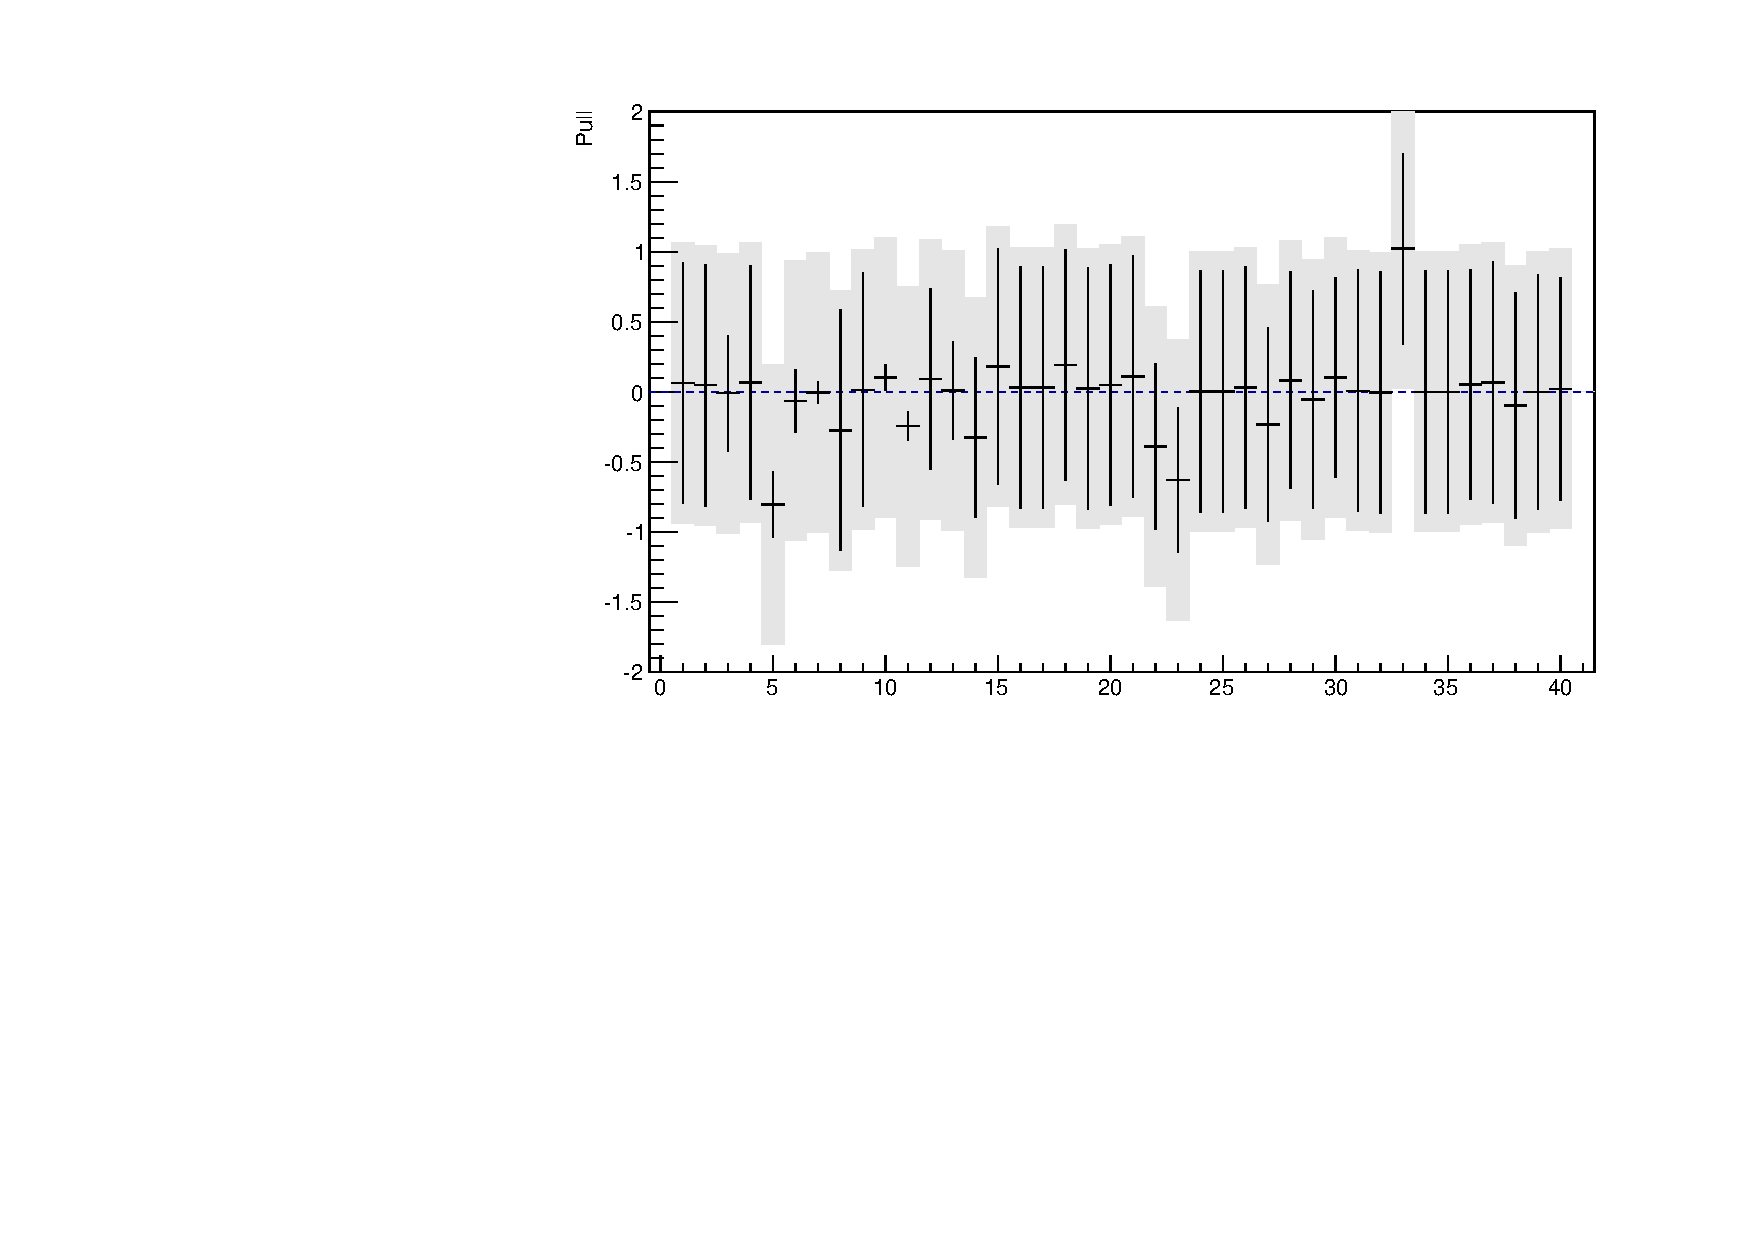
\includegraphics[width=1.0\textwidth]{figures/mlfit_Postnuisance_all_all.pdf}
}\\
\subfigure[]{
\centering
\label{subfig:Postnuisance_of_0j}
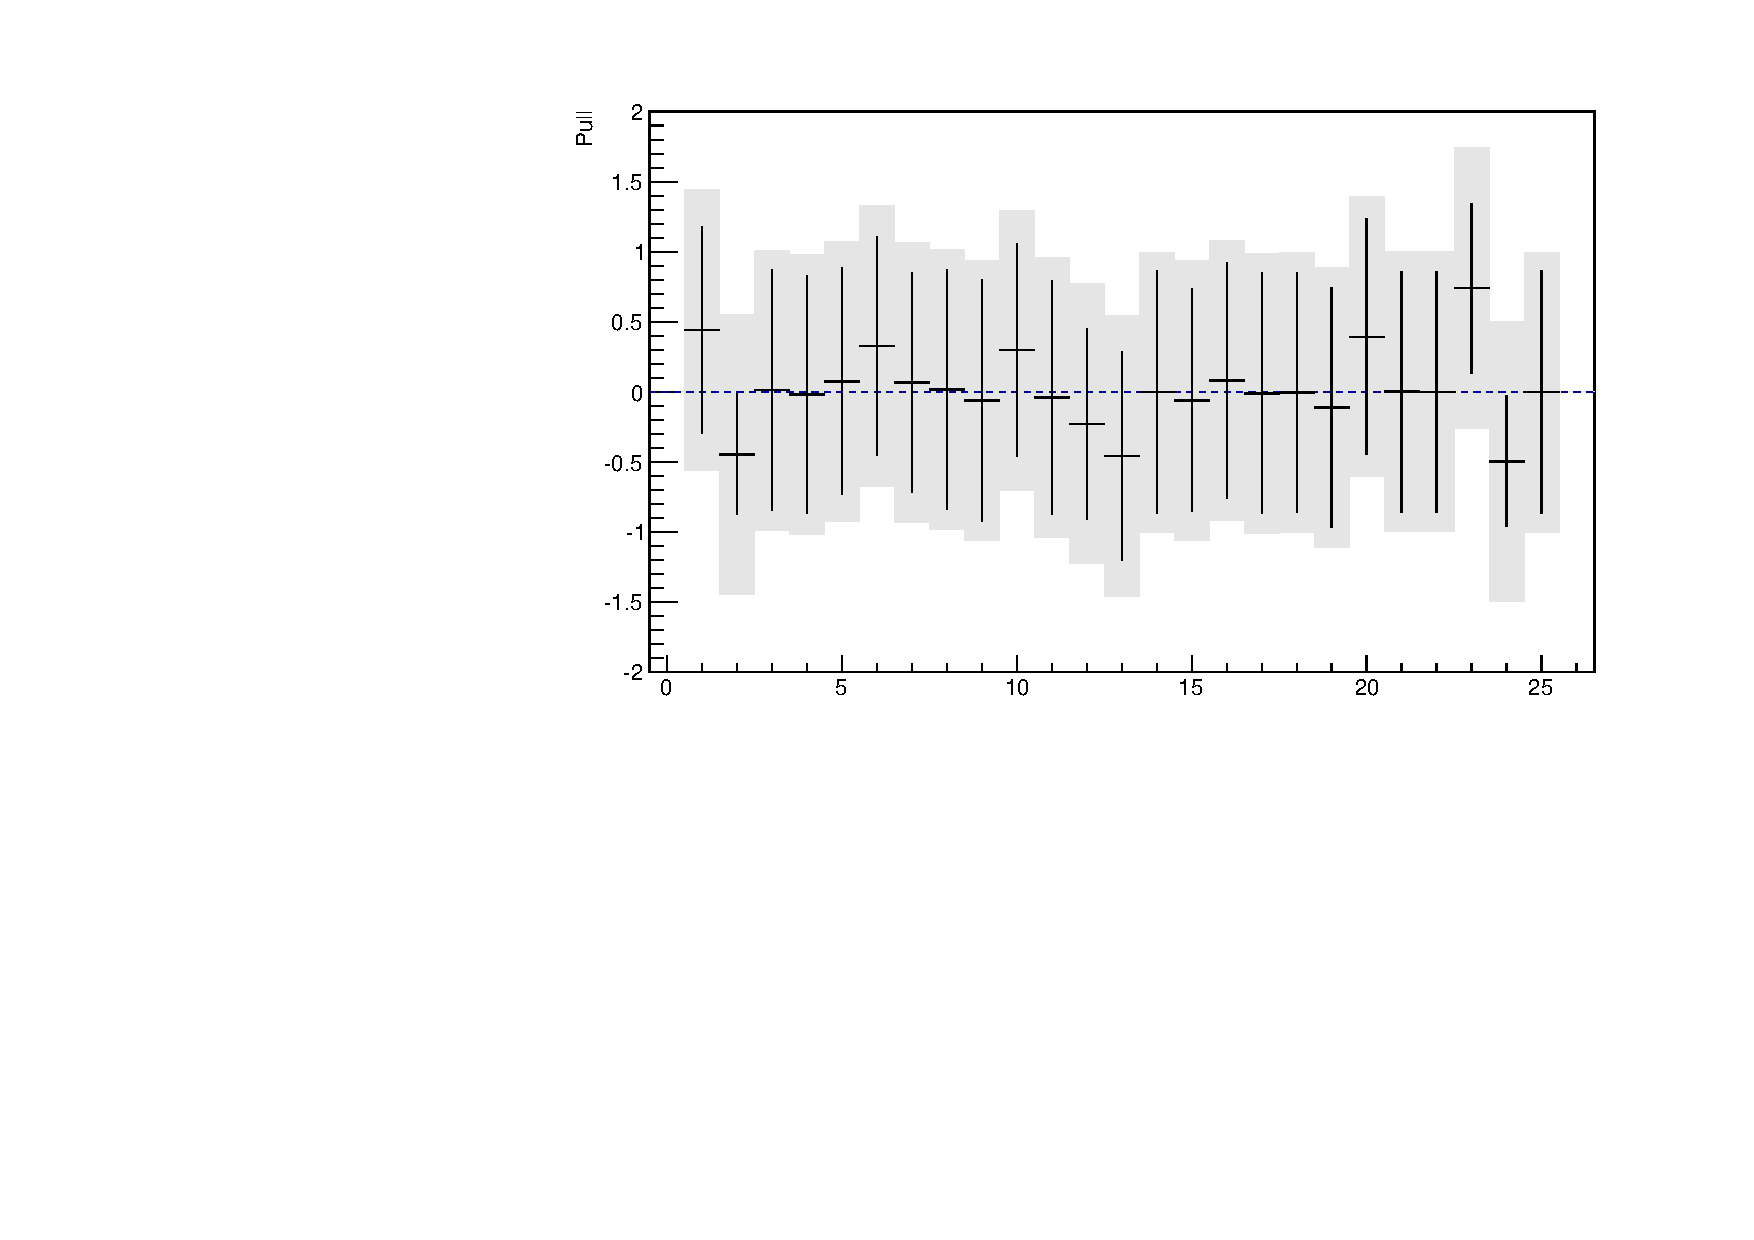
\includegraphics[width=.45\textwidth]{figures/mlfit_Postnuisance_of_0j.pdf}
}
\subfigure[]{
\centering
\label{subfig:Postnuisance_sf_0j}
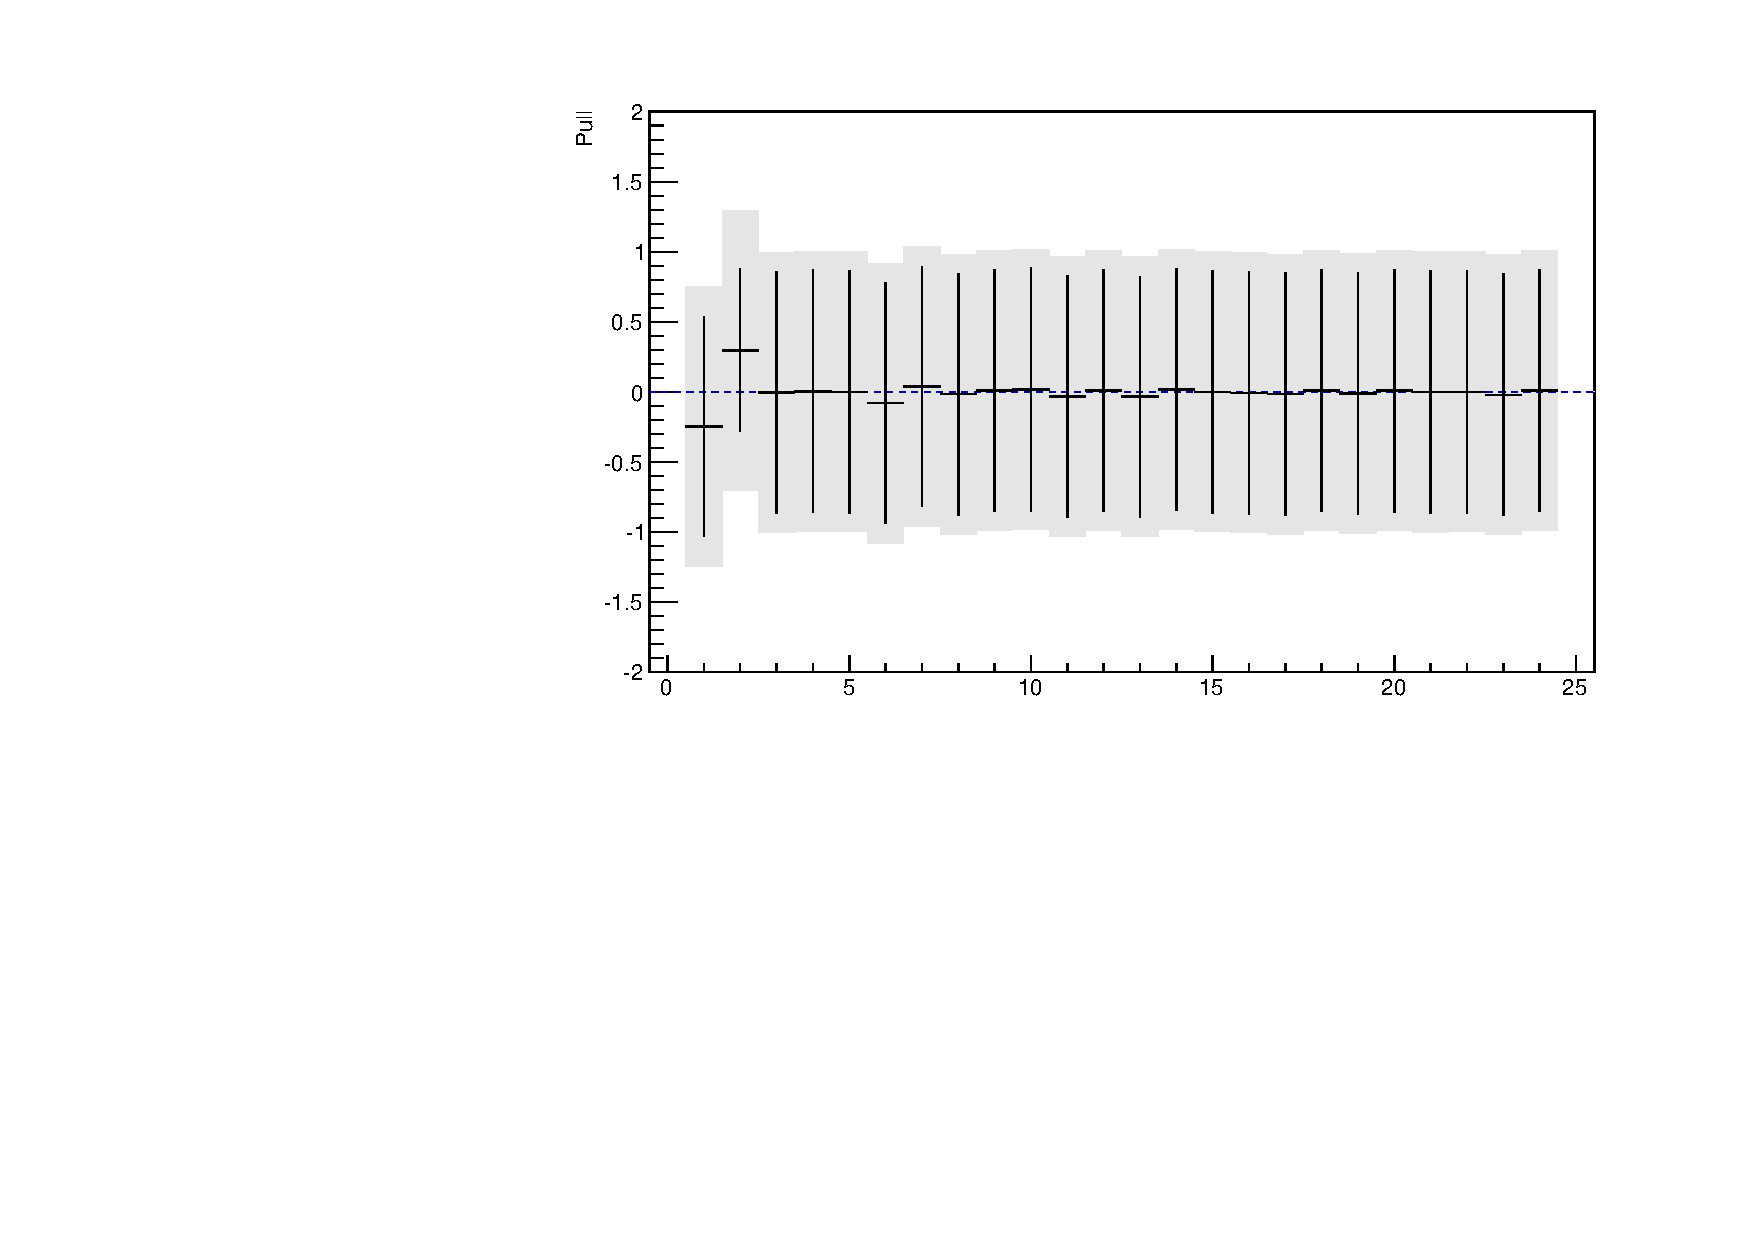
\includegraphics[width=.45\textwidth]{figures/mlfit_Postnuisance_sf_0j.pdf}
}
\subfigure[]{
\centering
\label{subfig:Postnuisance_of_1j}
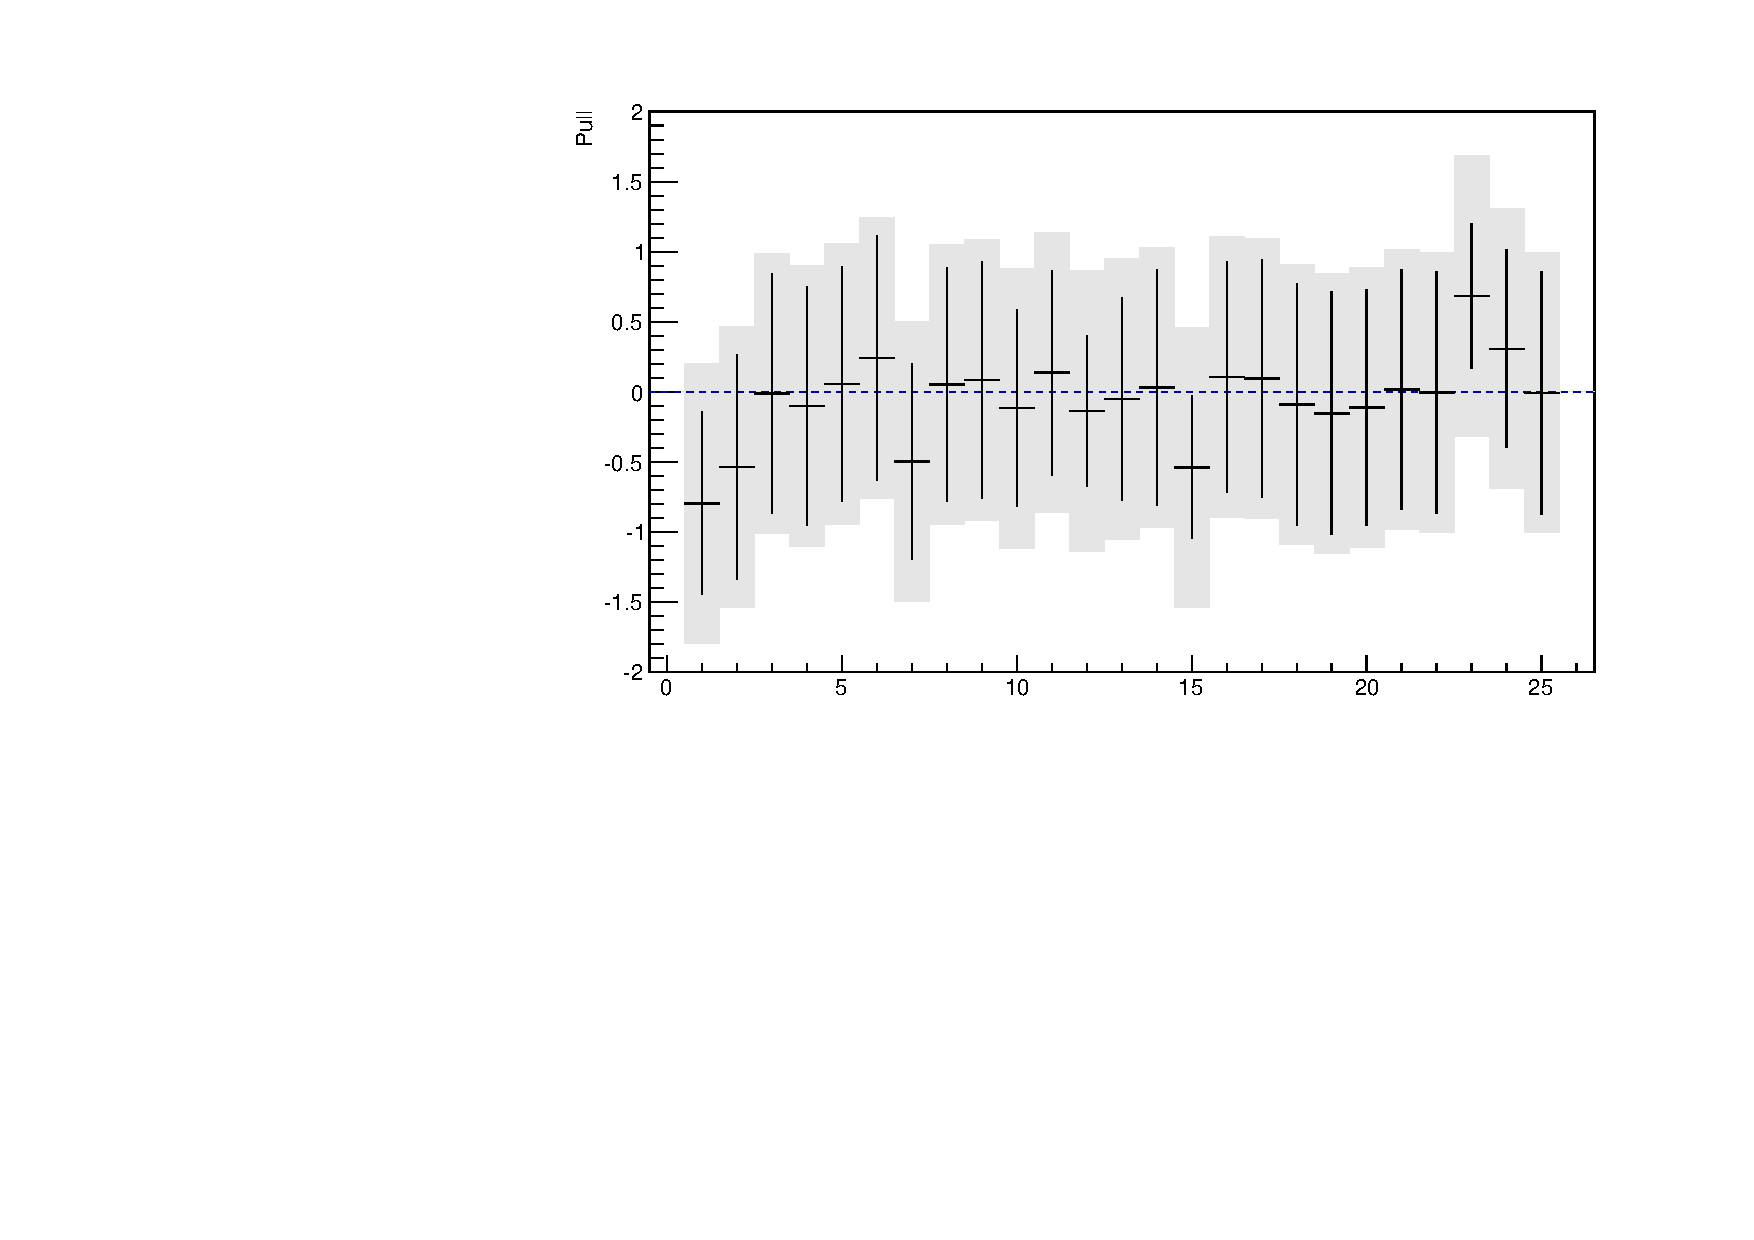
\includegraphics[width=.45\textwidth]{figures/mlfit_Postnuisance_of_1j.pdf}
}
\subfigure[]{
\centering
\label{subfig:Postnuisance_sf_1j}
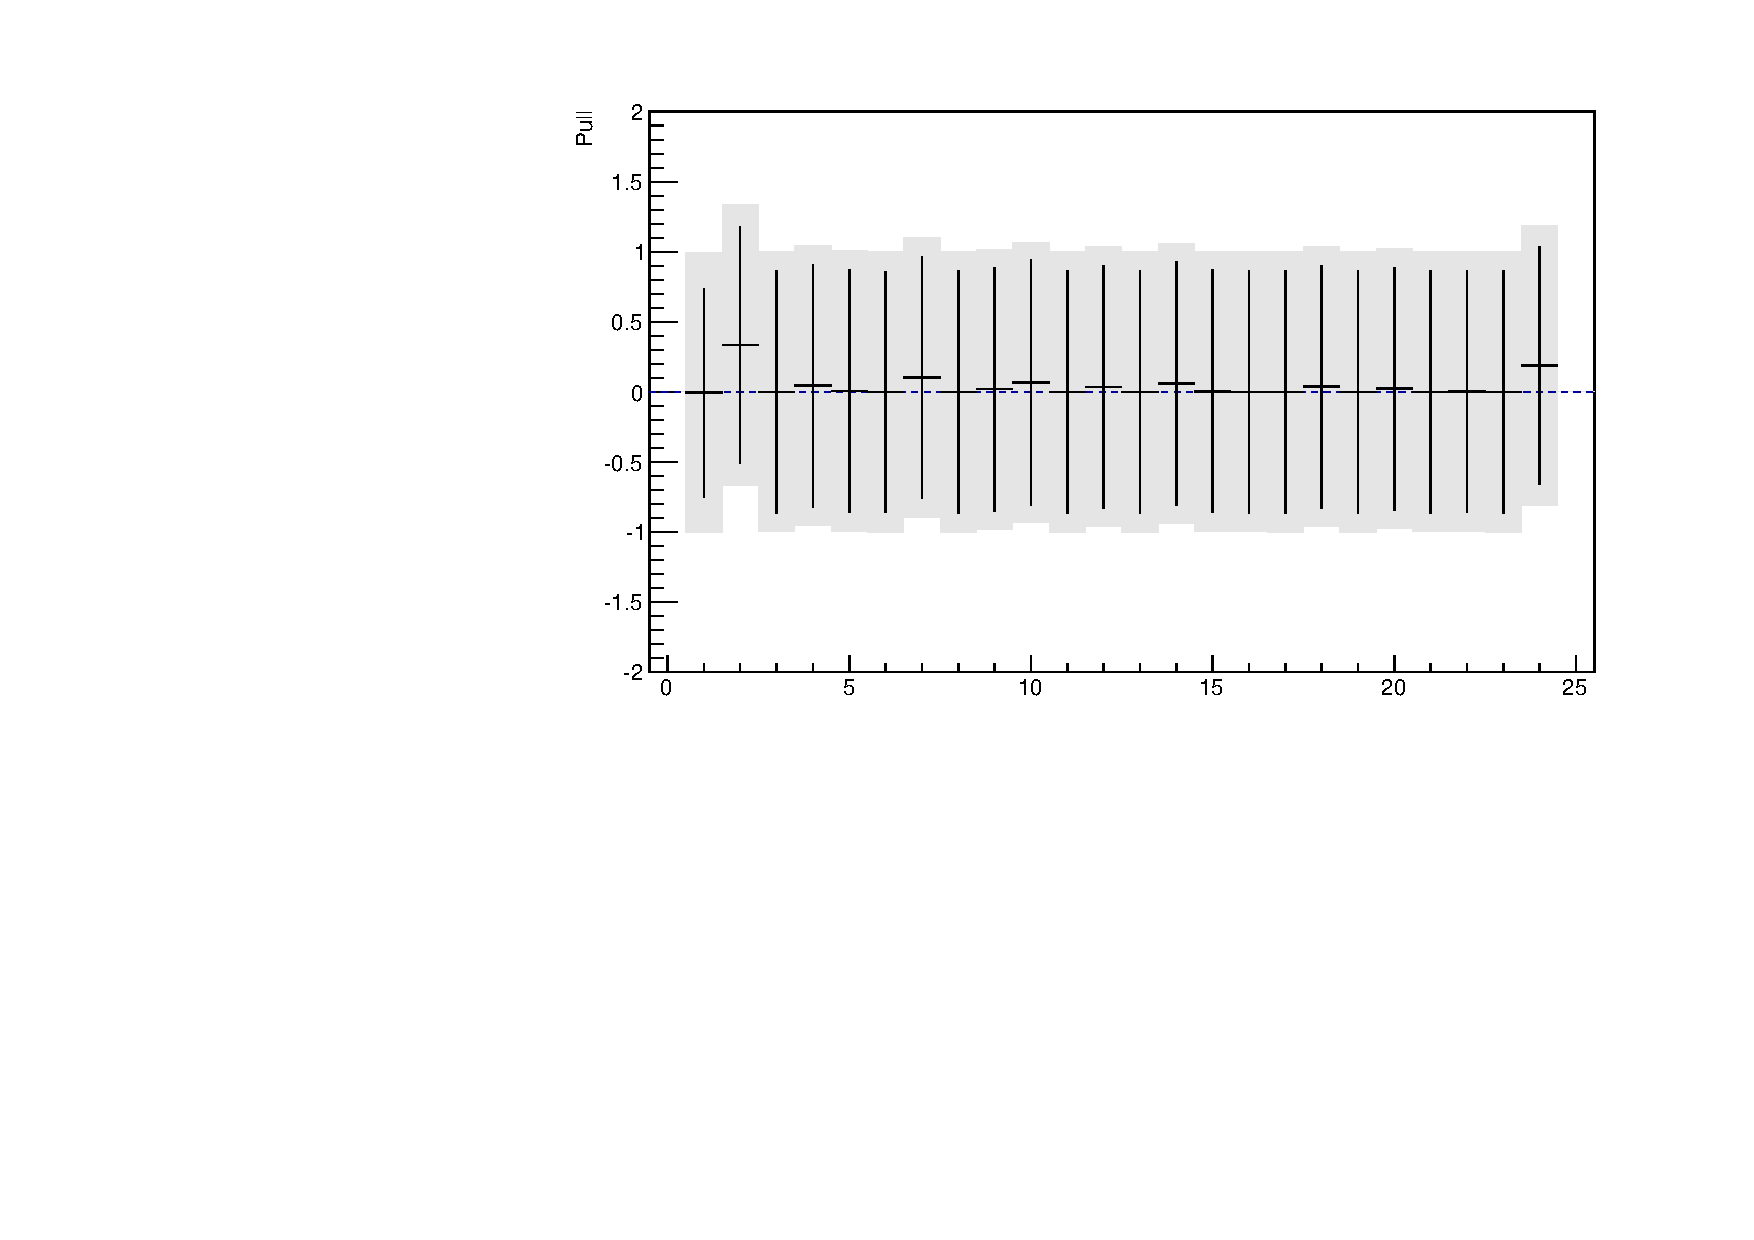
\includegraphics[width=.45\textwidth]{figures/mlfit_Postnuisance_sf_1j.pdf}
}
\caption{Post-fit results on the nuisance parameters.}
\label{fig:postnuisance}
\end{figure}
Figure~\ref{fig:postnuisance} shows the post-fit result of nuisance parameters. 
The x axis is the indices of the nuisance parameters, and the y axis is the 
Pull and the $\sigma_{\textrm{norm}}$. The black line shows the Pull 
as the central value and 
$\sigma_{\textrm{norm}}$ as an uncertainty bar. The grey area is drawn with the Pull as 
central value and the error bar being 1. This is drawn to visualize the size of 
the post-fit uncertainty with respect to the assigned uncertainty. 
The nuisances are divided into 5 groups; nuisances that are used (a) in all final states, 
(b) only in the \DF\ 0-jet category,  (c) only in the \SF\ 0-jet category,  
(d) only in the \DF\ 1-jet category,  and (e) only in the \SF\ 1-jet category. 

There is one nuisance parameter that has Pull greater than 1. 
But, it is one of the theory uncertainties on the \ggww process. 
Given that this process is not the dominant background process, 
and the exact value of Pull is 1.023, it does not affect the
result of the statistical interpretation.
There are several nuisances that have $\sigma_{\textrm{norm}}$ much 
less than 1. It is expected that $\sigma_{\textrm{norm}}$ can be less than 1, 
but at the same time we need to examine the over-constraining of 
those nuisances. 

%CMS_hww_MVALepResBounding  :     -0.804 +/-      0.234
%CMS_hww_MVAMETResBounding  :     -0.064 +/-      0.225
%CMS_hww_MVATopBounding     :     -0.003 +/-      0.081
%CMS_hww_MVAWWBounding      :      0.103 +/-      0.094
%CMS_hww_MVAWWNLOBounding   :     -0.244 +/-      0.101
There are 5 nuisance parameters that are constrained by more than 30 \%, 
\textit{i.e.} $\sigma_{\textrm{norm}}$ is less than 0.3. They are 
instrumental nuisances for lepton momentum resolution, \met\ resolution 
and alternate shape nuisances for \qqww\ and \topbkg.
The analysis is not designed to constrain the instrumental nuisances, 
thus some nuisances of this kind can be over-constrained allowing 
others nuisance not being constrained enough. In addition removing 
these nuisance from the statistical interpretation does 
change the results. In addition, we discussed that the fit model 
for  \qqww\ and \topbkg\ were validated using dedicated control regions.  
So, we conclude that the over-constraint of the these nuisances does 
not affect the final result. 

%\subsection{Correlations of nuisances}
%
%\textbf{Why look at correlations?} 
%\textcolor{red}{should have mentioned this way before}  
%
%The correlation between two nuisance parameters is quantified 
%using the linear correlation coefficient
%\begin{eqnarray} 
%\rho_{ij} = \frac{cov\left(\theta_i, \theta_j\right)}{\sigma_i \sigma_j}  
%\end{eqnarray} 
%where $cov\left(\theta_i, \theta_j\right)$ is the covariance of the  
%the two nuisance parameters, and $\sigma_{i(j)}$ is the variance 
%of the nuisance, $\theta_{i(j)}$.
%
%\begin{figure}[!hbtp]
%\centering
%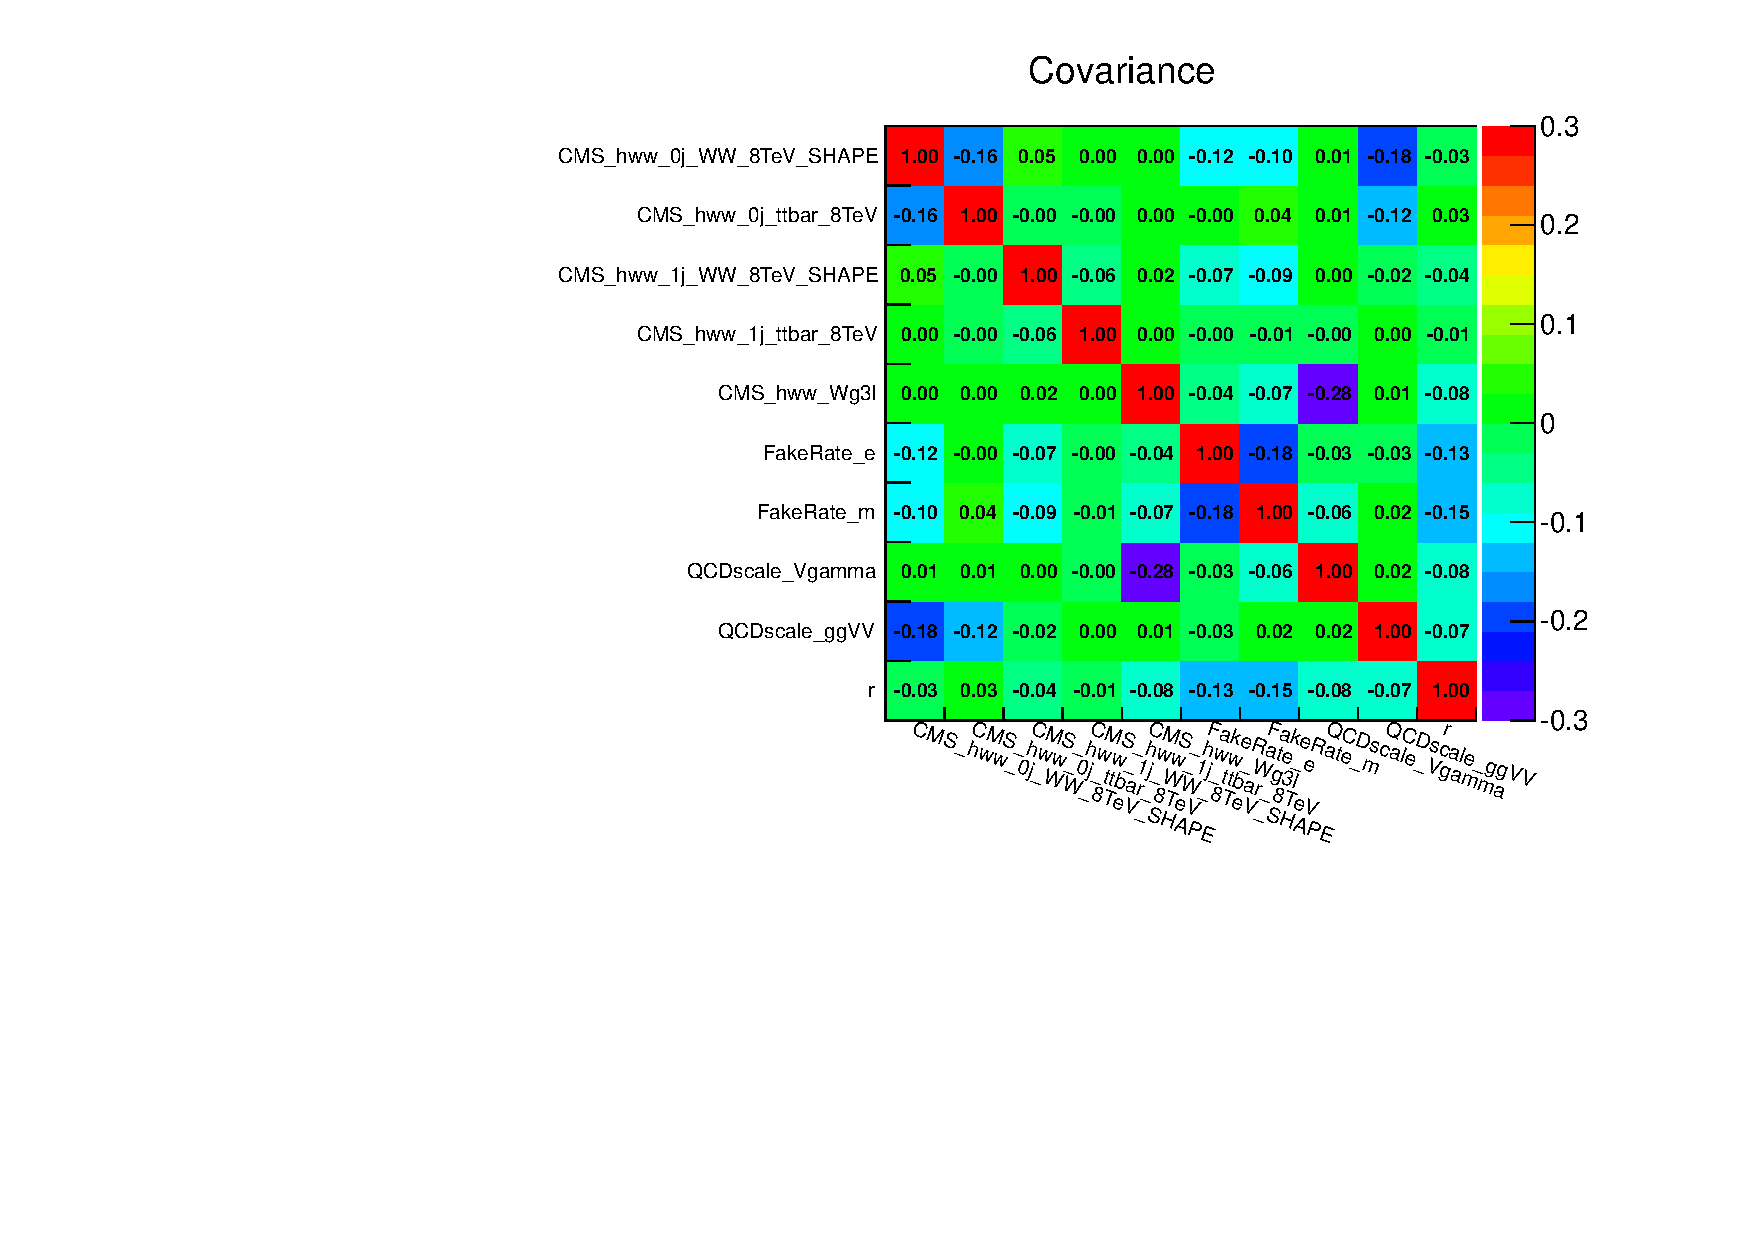
\includegraphics[width=1.0\textwidth]{figures/covariance.pdf}
%\caption{Correlation coefficients between the selective nuisance parameters.}
%\label{fig:covariance}
%\end{figure}
%
%%---------------------------------------------------------------------------------------------------------------------------------------------
%%    [ x, y] ==                                       Nuisance (X) :                                       Nuisance (Y) :          Correlation
%%---------------------------------------------------------------------------------------------------------------------------------------------
%%    [ 12, 97] ==                         CMS_hww_1j_WW_8TeV_SHAPE :               CMS_hwwof_1j_MVATopStatBounding_8TeV :            -0.513108
%%    [ 15, 75] ==                           CMS_hww_MVAJESBounding :              CMS_hwwof_1j_MVAqqWWStatBounding_8TeV :             0.591208
%%    [ 15, 97] ==                           CMS_hww_MVAJESBounding :               CMS_hwwof_1j_MVATopStatBounding_8TeV :            -0.913373
%%    [ 15, 133] ==                          CMS_hww_MVAJESBounding :                             CMS_hww_MVATopBounding :             0.994357
%%    [ 19, 75] ==                           CMS_hww_MVATopBounding :              CMS_hwwof_1j_MVAqqWWStatBounding_8TeV :             0.594662
%%    [ 19, 97] ==                           CMS_hww_MVATopBounding :               CMS_hwwof_1j_MVATopStatBounding_8TeV :            -0.918617
%%    [ 55, 75] ==             CMS_hwwof_1j_MVATopStatBounding_8TeV :              CMS_hwwof_1j_MVAqqWWStatBounding_8TeV :              -0.6451
%%---------------------------------------------------------------------------------------------------------------------------------------------
%
%Figure~\ref{fig:covariance} shows the correlation coefficients
%of selective nuisances which are normalization uncertainties of dominant processes. 
%Here is the list of the nuisances and their meainings. 
%\begin{itemize} 
%\item \verb|CMS_hww_0j_WW_8TeV_SHAPE|  \\ 
%     normalization of \qqww\ in \DF\ 0-jet 8TeV with flat prior
%\item \verb|CMS_hww_0j_ttbar_8TeV|  \\
%     normalization of \topbkg\ in 0-jet 8TeV with log normal prior
%\item \verb|CMS_hww_1j_WW_8TeV_SHAPE|  \\ 
%     normalization of \qqww\ in \DF\ 1-jet 8TeV with flat prior 
%\item \verb|CMS_hww_1j_ttbar_8TeV|  \\ 
%     normalization of \topbkg\ in 1-jet 8TeV with log normal prior
%\item \verb|CMS_hww_Wg3l|  \\
%     normalization of \wgammastar\ with log normal prior
%\item \verb|QCDscale_Vgamma|  \\
%     normalization of \wgamma\ with log normal prior 
%\item \verb|QCDscale_ggVV|  \\
%     normalization of \ggww\ with log normal prior 
%\item \verb|FakeRate_e|  \\
%     normalization of \WjetsE\ with log normal prior
%\item \verb|FakeRate_m|  \\
%     normalization of \WjetsM\ with log normal prior 
%\item \verb|r|  \\
%     signal strength with flat prior 
%\end{itemize}
%
%
%
\subsection{Post-fit Result of Normalization} 

In this section we check if there is any process of which post-fit 
normalization changes dramatically. A large variation which touches 
the boundary of the allowed uncertainty range might indicate that 
the fit model is not correct. 

\begin{table}[ht!]
\begin{center}
\begin{tabular}{c|cc|cc}
\hline
\hline
        Process &    N(prefit) &   N(postfit) & Difference(raw) &  Difference(\%)  \\  
\hline
\hline
          \qqZH &        1.7 &        1.3 &       -0.4 &      -23.9        \\
          \qqWH &        5.7 &        4.5 &       -1.2 &      -20.4        \\
           \qqH &        2.9 &        2.2 &       -0.7 &      -23.9        \\
           \ggH &      228.1 &      169.6 &      -58.5 &      -25.6        \\
\hline
          \qqww &     3981.7 &     3935.7 &      -46.0 &       -1.2        \\
          \ggww &      211.3 &      292.1 &       80.8 &       38.3        \\
            \vv &      132.6 &      132.2 &       -0.4 &       -0.3        \\
        \topbkg &      499.4 &      422.9 &      -76.4 &      -15.3        \\
        \WjetsE &      284.7 &      250.6 &      -34.1 &      -12.0        \\
        \wgamma &      115.6 &      107.8 &       -7.7 &       -6.7        \\
    \wgammastar &      130.7 &      119.0 &      -11.7 &       -8.9        \\
           \ztt &       46.0 &       47.2 &        1.3 &        2.7        \\
        \WjetsM &      332.2 &      249.0 &      -83.2 &      -25.0        \\
\hline
\hline
\end{tabular}
\caption{The pre-fit and post-fit normalizations in \DF\ 0-jet category in 8~\TeV.}
\label{tab:postfitnorm_of0j8tev}
\end{center}
\end{table}

\begin{table}[ht!]
\begin{center}
\begin{tabular}{c|cc|cc}
\hline
\hline
        Process &    N(prefit) &   N(postfit) & Difference(raw) &  Difference(\%)  \\  
\hline
\hline
          \qqZH &        1.9 &        1.5 &       -0.4 &      -21.7        \\
          \qqWH &        6.9 &        5.4 &       -1.5 &      -21.8        \\
           \qqH &       11.1 &        8.5 &       -2.7 &      -24.0        \\
           \ggH &       88.5 &       68.8 &      -19.8 &      -22.3        \\
\hline
          \qqww &     1203.1 &     1279.0 &       75.9 &        6.3        \\
          \ggww &       69.0 &       88.4 &       19.4 &       28.1        \\
            \vv &      116.6 &      114.8 &       -1.8 &       -1.6        \\
        \topbkg &     1436.8 &     1348.7 &      -88.1 &       -6.1        \\
        \WjetsE &      130.4 &      120.0 &      -10.4 &       -8.0        \\
        \wgamma &       29.1 &       27.7 &       -1.3 &       -4.6        \\
    \wgammastar &       20.0 &       11.1 &       -8.9 &      -44.5        \\
           \ztt &       76.8 &       78.9 &        2.2 &        2.9        \\
        \WjetsM &      153.0 &      124.0 &      -29.0 &      -19.0        \\
\hline
\hline
\end{tabular}
\caption{The pre-fit and post-fit normalizations in \DF\ 1-jet category in 8~\TeV.}
\label{tab:postfitnorm_of1j8tev}
\end{center}
\end{table}

\begin{table}[ht!]
\begin{center}
\begin{tabular}{c|cc|cc}
\hline
\hline
        Process &    N(prefit) &   N(postfit) & Difference(raw) &  Difference(\%)  \\  
\hline
\hline
          \qqZH &        0.1 &        0.1 &       -0.0 &      -23.4        \\
          \qqWH &        0.5 &        0.4 &       -0.1 &      -23.4        \\
           \qqH &        0.5 &        0.4 &       -0.1 &      -23.4        \\
           \ggH &       55.8 &       41.9 &      -13.9 &      -25.0        \\
\hline
          \qqww &      197.6 &      201.1 &        3.5 &        1.8        \\
          \ggww &        9.8 &       12.9 &        3.2 &       32.3        \\
            \vv &       13.3 &       13.4 &        0.1 &        0.7        \\
        \topbkg &        9.3 &        8.8 &       -0.5 &       -5.8        \\
         \Zjets &       92.2 &      100.5 &        8.3 &        9.0        \\
        \WjetsE &       12.4 &       12.6 &        0.2 &        1.6        \\
        \wgamma &        3.2 &        3.1 &       -0.1 &       -4.5        \\
    \wgammastar &        5.1 &        4.6 &       -0.5 &       -9.7        \\
        \WjetsM &       16.5 &       17.1 &        0.6 &        3.7        \\
\hline
\hline
\end{tabular}
\caption{The pre-fit and post-fit normalizations in \SF\ 0-jet category in 8~\TeV.}
\label{tab:postfitnorm_sf0j8tev}
\end{center}
\end{table}

\begin{table}[ht!]
\begin{center}
\begin{tabular}{c|cc|cc}
\hline
\hline
        Process &    N(prefit) &   N(postfit) & Difference(raw) &  Difference(\%)  \\  
\hline
\hline
          \qqZH &        0.3 &        0.2 &       -0.1 &      -22.9        \\
          \qqWH &        0.7 &        0.5 &       -0.2 &      -22.9        \\
           \qqH &        2.1 &        1.6 &       -0.5 &      -23.0        \\
           \ggH &       15.9 &       12.6 &       -3.3 &      -20.6        \\
\hline
          \qqww &       37.8 &       39.6 &        1.8 &        4.8        \\
          \ggww &        2.2 &        3.0 &        0.8 &       36.1        \\
            \vv &        6.5 &        6.6 &        0.1 &        1.7        \\
        \topbkg &       40.4 &       40.9 &        0.5 &        1.2        \\
         \Zjets &       14.7 &       16.3 &        1.6 &       10.8        \\
        \WjetsE &        2.8 &        2.9 &        0.1 &        2.3        \\
        \wgamma &        2.5 &        2.4 &       -0.1 &       -2.1        \\
    \wgammastar &        0.7 &        0.6 &       -0.1 &       -8.4        \\
        \WjetsM &        3.7 &        3.9 &        0.2 &        4.8        \\
\hline
\hline
\end{tabular}
\caption{The pre-fit and post-fit normalizations in \SF\ 1-jet category in 8~\TeV.}
\label{tab:postfitnorm_sf1j8tev}
\end{center}
\end{table}

\begin{table}[ht!]
\begin{center}
\begin{tabular}{c|cc|cc}
\hline
\hline
        Process &    N(prefit) &   N(postfit) & Difference(raw) &  Difference(\%)  \\  
\hline
\hline
           \qqH &        0.4 &        0.3 &       -0.1 &      -23.6        \\
           \ggH &       50.3 &       37.6 &      -12.8 &      -25.4        \\
\hline
          \qqww &      828.8 &      810.5 &      -18.3 &       -2.2        \\
          \ggww &       40.8 &       52.7 &       11.9 &       29.3        \\
            \vv &       17.7 &       17.8 &        0.1 &        0.6        \\
        \topbkg &       91.2 &       99.1 &        7.9 &        8.7        \\
         \Zjets &        4.9 &        4.6 &       -0.4 &       -7.2        \\
        \WjetsE &       88.3 &       84.4 &       -3.9 &       -4.4        \\
        \wgamma &       19.7 &       18.6 &       -1.1 &       -5.5        \\
    \wgammastar &       36.4 &       35.9 &       -0.5 &       -1.5        \\
        \WjetsM &       62.7 &       45.8 &      -17.0 &      -27.0        \\
\hline
\hline
\end{tabular}
\caption{The pre-fit and post-fit normalizations in \DF\ 0-jet category in 7~\TeV.}
\label{tab:postfitnorm_of0j7tev}
\end{center}
\end{table}

\begin{table}[ht!]
\begin{center}
\begin{tabular}{c|cc|cc}
\hline
\hline
        Process &    N(prefit) &   N(postfit) & Difference(raw) &  Difference(\%)  \\  
\hline
\hline
           \qqH &        2.1 &        1.6 &       -0.5 &      -23.5        \\
           \ggH &       17.1 &       13.6 &       -3.5 &      -20.6        \\
\hline
          \qqww &      246.3 &      273.6 &       27.3 &       11.1        \\
          \ggww &       14.0 &       17.7 &        3.7 &       26.5        \\
            \vv &       18.1 &       18.1 &       -0.0 &       -0.0        \\
        \topbkg &      226.7 &      203.9 &      -22.8 &      -10.0        \\
         \Zjets &        8.3 &        3.2 &       -5.1 &      -61.3        \\
        \WjetsE &       34.4 &       28.5 &       -5.9 &      -17.1        \\
        \wgamma &        3.6 &        3.4 &       -0.2 &       -4.3        \\
    \wgammastar &        4.8 &        5.0 &        0.2 &        3.5        \\
        \WjetsM &       26.2 &       19.2 &       -7.0 &      -26.7        \\
\hline
\hline
\end{tabular}
\caption{The pre-fit and post-fit normalizations in \DF\ 1-jet category in 7~\TeV.}
\label{tab:postfitnorm_of1j7tev}
\end{center}
\end{table}

\begin{table}[ht!]
\begin{center}
\begin{tabular}{c|cc|cc}
\hline
\hline
        Process &    N(prefit) &   N(postfit) & Difference(raw) &  Difference(\%)  \\  
\hline
\hline
           \qqH &        0.1 &        0.1 &       -0.0 &      -22.9        \\
           \ggH &       10.0 &        7.5 &       -2.5 &      -24.7        \\
\hline
          \qqww &       45.0 &       44.5 &       -0.4 &       -1.0        \\
          \ggww &        2.0 &        2.6 &        0.6 &       28.9        \\
            \vv &        0.9 &        0.9 &        0.0 &        1.3        \\
        \topbkg &        2.0 &        2.0 &       -0.0 &       -0.3        \\
         \Zjets &       10.6 &        9.7 &       -0.9 &       -8.2        \\
        \WjetsE &        2.1 &        2.2 &        0.0 &        0.9        \\
    \wgammastar &        0.7 &        0.7 &       -0.1 &       -9.8        \\
        \WjetsM &        1.0 &        1.1 &        0.0 &        1.9        \\
\hline
\hline
\end{tabular}
\caption{The pre-fit and post-fit normalizations in \SF\ 0-jet category in 7~\TeV.}
\label{tab:postfitnorm_sf0j7tev}
\end{center}
\end{table}

\begin{table}[ht!]
\begin{center}
\begin{tabular}{c|cc|cc}
\hline
\hline
        Process &    N(prefit) &   N(postfit) & Difference(raw) &  Difference(\%)  \\  
\hline
\hline
           \qqH &        0.4 &        0.3 &       -0.1 &      -22.5        \\
           \ggH &        2.6 &        2.1 &       -0.5 &      -20.1        \\
\hline
          \qqww &        9.7 &        9.9 &        0.1 &        1.5        \\
          \ggww &        0.7 &        0.9 &        0.2 &       32.0        \\
            \vv &        0.7 &        0.7 &        0.0 &        1.9        \\
        \topbkg &        6.4 &        6.3 &       -0.1 &       -1.4        \\
         \Zjets &        9.8 &        9.8 &       -0.0 &       -0.2        \\
        \WjetsE &        0.7 &        0.7 &        0.0 &        1.6        \\
    \wgammastar &        0.2 &        0.2 &       -0.0 &       -8.8        \\
        \WjetsM &        0.2 &        0.2 &        0.0 &        3.4        \\
\hline
\hline
\end{tabular}
\caption{The pre-fit and post-fit normalizations in \SF\ 1-jet category in 7~\TeV.}
\label{tab:postfitnorm_sf1j7tev}
\end{center}
\end{table}

Tables~\ref{tab:postfitnorm_of0j8tev} - \ref{tab:postfitnorm_sf1j7tev} show 
the pre-fit and post-fit normalizations of each process, and the difference 
in absolute yield and relative fraction in \%, in each categories. In general 
most of the processes are stable, but \ggww has a large change. This is driven 
by the nuisance, \verb|QCDscale_ggVV|, which was pulled by 1$\sigma$. 
This nuisance is anti-correlated with those of \qqww\ and \topbkg, 
which are moved down by the fit. Given that this background is small, 
and its shape is different from that of signal, this does not 
affect the result of statistical interpretation.





